%Main Document
\documentclass[a4paper, 11pt, oneside]{AuProjectHandin}
\usepackage{titlesec}
\usepackage{AuPreamble}
%configurationfile
\pagestyle{AuHandin}

\title{Process Rapport}
%author will mostly not be used unless we are talking solo work and then group members should be disabled ;)
\author{Forfatter Navn}
%Vejlederens navn
\SetVejleder{Søren Hansen}
%Skole/Universitetets navn
\SetUniversity{Aarhus Universitet}
%Projektnavn
\SetProject{Semesterprojekt 3. Semester}
%Gruppe Nummer
\SetGroupNumber{10}
%Add the names of all the members in the group, can handle 1 to 8 members, names are added one per set of []
\GroupMemberNames[Tonni Nybo Follmann][Stefan Nielsen][Mikkel Espersen][Halfdan Vanderbruggen Bjerre][Ahmad Sabah][Jacob Munkholm Hansen]{}
%add student numbers of the students, must have the exact same order as the names listed above.
\GroupMemberStudentNo[201504573][201508282][201507348][20091153][201209619][201404796]{}
\newcommand{\myparagraph}[1]{\paragraph{#1}\mbox{}\\}
\newcommand{\mysubparagraph}[1]{\noindent\subparagraph{#1}\mbox{}\\}
%\titleformat*{\chapter}{\LARGE\bfseries}
\titleformat*{\section}{\LARGE\bfseries}
\titleformat*{\subsection}{\Large\bfseries}
\titleformat*{\subsubsection}{\large\bfseries}
\begin{document}

%titlepage
\begin{titlingpage}
	\center
	\HUGE\thetitle
	
	
	\LARGE\ShowProject
	
	\Large Gruppe \ShowGroupNumber
	
	
	
	\normalsize Vejleder: \ShowVejleder
	
	Gruppemedlemmer:
	
	\PrintGroupMembers
\end{titlingpage}

\begin{figure}[H]
	\centerline{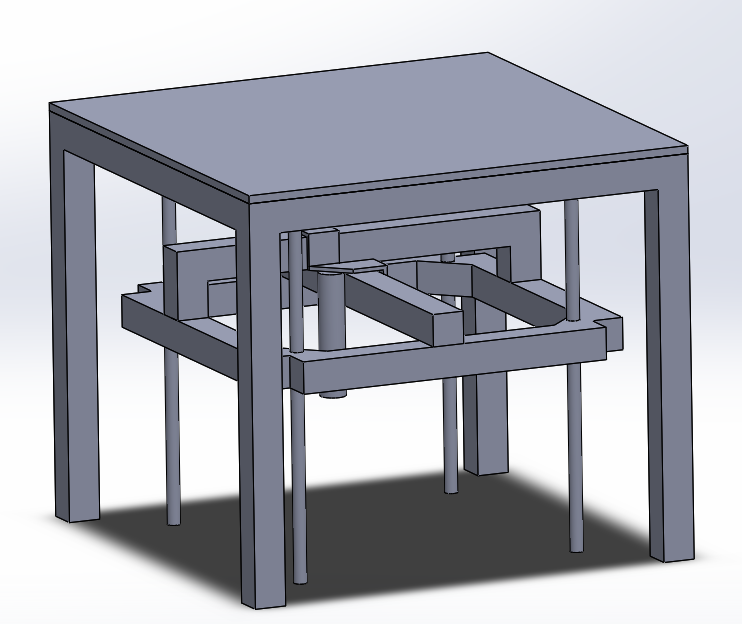
\includegraphics[scale=0.07]{winePrep}}
	\caption{winePrep}
\end{figure}
\frontmatter
\tableofcontents
\mainmatter

\chapter{Forord}
Denne rapport er skrevet på 3. semester af gruppe 10, på retningerne IKT og EE ved Aarhus Universitet, Ingeniørhøjskolen.
Vejleder for dette projekt er Søren Hansen. Afleveringsdatoen for denne projektrapport er den 20. december 2016, og bedømmelse er den 18. januar 2017.
Rapporten er udarbejdet på baggrund af den dokumentation, som kan findes i bilaget for projektrapporten.

\section{Læsevejledning}
Rapporten er inddelt i nummererede kapitler. Hvert kapitel indeholder nummererede sektioner med dertil hørende undersektioner. Nedenunder er givet eksempler på disse. \\

\begin{figure}[H]
	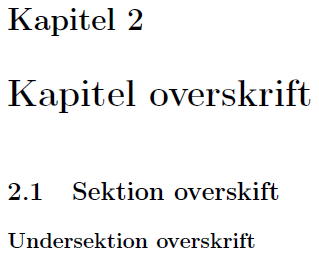
\includegraphics{KapitelStoerrelse.png}
\end{figure}

\noindent
Der vil blive brugt initialer på gruppens medlemmer til angivelse af, hvem rapportens sektioner er skrevet af: \\
\\
Mikkel Busk Espersen (MBE), \\
Jacob Munkholm Hansen(JMH), \\
Ahmad Sabah (AS), \\
Halfdan Vanderbruggen Bjerre(HVB). \\
\\
I de udarbejdede UML- og SysML-diagrammer og beskrivelser af disse vil der blive refereret til p- og s-motorer. Disse dækker over motorerne til styring af 
henholdsvis åbningsmekanismen\footnote{Se ordliste i bilag} og skruen.

\section{Hovedansvarsområder}
Tabel \ref{tab:ansvar} viser fordelingen af hovedansvarsområder for produktet fordelt på gruppemedlemmer. Emnerne er inddelt i primær og sekundær, som informerer om 
medlemmers specialistviden og kernekompetencer indenfor produktudviklingen. Enkelte sekundære felter er tomme, dette betyder at ingen har været sekundær på 
emnet.

\begin{table}[H]
	\centering
	\begin{tabular}{| l | c | c |}
		\hline
		Emne & Primær & Sekundær\\\hline
		Brugergrænseflade (GUI) & AS & HVB\\\hline
		SPI DevKit-PSoC & HVB & JMH\\\hline
		SPI PSoC-PSoC & HVB, JMH & \\\hline
		PSoC software sensor & JMH & MBE\\\hline
		PSoC software sensor & JMH & MBE\\\hline
		Bipolære motorer & MBE & JMH\\\hline
		Unipolære motorer & MBE & JMH\\\hline
		DC motor & MBE & \\\hline
		Konstruktion og mekanik & AS & HVB\\\hline
	\end{tabular}
	\caption{Fordeling af hovedansvarsområder}
	\label{tab:ansvar}
\end{table}
\chapter{Indledning}
\section{Projektformulering}
Mange ældre har i dag svært ved at åbne deres vinflaske, da de ikke har den fornødne styrke til selv at trække korkproppen ud af vinflasken. Derfor vil det være ideelt for dem, at have en løsning hvor åbningen af vinflaskerne bliver automatiseret.

For at få den optimale oplevelse ud af en vin, skal den åbnes rettidigt så den iltes før indtagelse. Iltningstiden kan variere fra vin til vin, og derfor kan mange uerfarne vindrikkere have svært ved at ilte deres vin korrekt. Mange glemmer at åbne vinen i god tid, og opnår derfor ikke den optimale oplevelse. Det kan derfor være ideelt, hvis denne proces også automatiseres.

\begin{figure}[H]
	\caption{Rigt billede der beskriver WinePrep}
	\label{RIGTBILLEDE}
	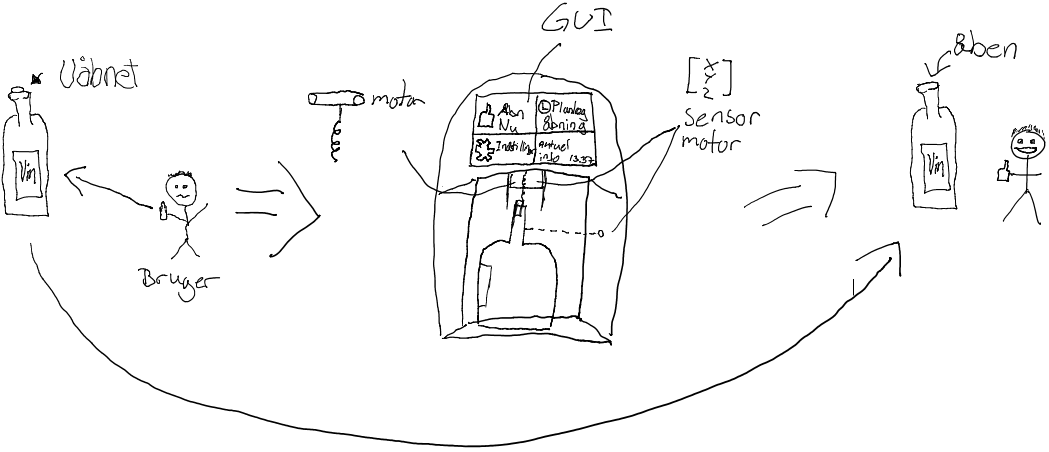
\includegraphics[scale=0.6]{WinePrep_realistisk.png}
\end{figure}

\section{Det realistiske system}
WinePrep er den automatiske vinåbner som er illustreret på Figur \ref{RIGTBILLEDE}, hvilket beskriver det realistiske system i en tænkt situation. Der er siden udarbejdelsen af det rige billede ikke ændret ved tanken bag systemets funktionalitet, blot andre måder at implementere ideerne på.\\

Den oprindelige tanke med WinePrep gør det for brugeren muligt at åbne en bestemt type vinflaske ved at indsætte vinen i maskinen, konfigurere WinePrep til at åbne og derefter først lade systemet lokalisere flasken hvorefter en åbningsmekanisme sænker sig over vinen og trækker korkproppen op. Dette realiseres med WinePreps ramme, brugergrænseflade, sensorer, aktuatorer og proptrækker samt microcontrollere til at lade systemet kommunikere internt.

På baggrund af de tekniske komponenter og WinePreps kompleksitet, vil der til udviklere være krav om forhåndskendskab til elektronik og programmering, på et plan der gør det muligt at forstå og bruge de oplysninger der findes i bilagene til denne rapport.

WinePrep er en prototype der er mulig at udvikle og optimere på.

\section{Hovedansvarsområder}
Tabel xx viser fordelingen af hovedansvarsområder for produktet fordelt på gruppemedlemmer. Emnerne er inddelt i primær og sekundær, som informerer om medlemmers specialistviden og kernekompetencer indenfor produktudviklingen. Enkelte sekundære felter er tomme, dette betyder at ingen har været sekundær på emnet.\\

\begin{tabular}{| l | c | c |}
\hline
Emne & Primær & Sekundær\\\hline
Brugergrænseflade (GUI) & AS & HVB\\\hline
SPI DevKit-PSoC & HVB & JMH\\\hline
SPI PSoC-PSoC & HVB, JMH & \\\hline
PSoC software sensor & JMH & MBE\\\hline
PSoC software sensor & JMH & MBE\\\hline
Bipolære motorer & MBE & JMH\\\hline
Unipolære motorer & MBE & JMH\\\hline
DC motor & MBE & \\\hline
Konstruktion og mekanik & AS & HVB\\\hline
\end{tabular}
\chapter{Afgrænsning}
Det er fra IHA's side opstillet følgende krav til projektet:\\
- Der skal indgå en aktuator og/eller sensor.
- Der skal være implementeret en brugergrænseflade.
- PSoC og Linux platform skal indgå i projektet.
- Skal indeholde faglige elementer fra semesterets andre fag.

En afgrænsning for projektet er formuleret ud fra visionen for winePrep. Tilkobling af winePrep til database, den mobile applikation, samt regulering af vinens 
temperatur, anses for spændende udfordringer, dog en anelse for tidskrævende. Desuden ligger disse funktioner uden for de faglige mål for projektet, og vil 
derfor ikke blive medtaget. Implementeringen af et socialt medie som "winebook" er meget omfangsrigt, og er ikke realistisk for dette projekt.\\

Hovedfunktionalitet for systemet er åbning af en vinflaske, og denne funktionalitet ønskes derfor med i projektet. Herudover bliver timing af åbningstidspunkt 
og detektering af vinflaskens position udvalgt som realistisk mål for dette projekt. Dispensering af korkproppen bliver også medtaget, men simplificeret så denne
process blot består i at rotere skruen den modsatte vej, og dermed lade proppen falde af.\\

Projektet skal gerne udmunde i en prototype med ovenstående funktionalitet, som kan bruges til videreudvikling. Den endelige prototype vil ikke fremstå som et 
færdigt produkt, hverken i funktionalitet eller konstruktion. 

    
\chapter{Krav}
I henhold til projektets mål er der med udgangspunkt i FURPS+(indsæt reference til beskrivelse af FURPS+) og MoSCoW(indsæt reference til beskrivelse af MoSCoW) blevet opstillet en række krav for WinePrep. De funktionelle krav er beskrevet ved tre use-cases, hvoraf de to mest betydende for WinePrep's værdi vil blive beskrevet nøjere i dette kapitel. Disse omfatter den essentielle funktionalitet, som gør WinePrep enestående i forhold til andre produkter på markedet. Før disse beskrives er det dog påliggende at få sat nogle rammer på WinePrep i form af systemets grænseflader til dettes aktører.

\section{Aktører}
Der er to aktører for dette system: brugeren af WinePrep; og den givne vinflaske, der skal åbnes.

\subsection{Bruger}
Brugeren af WinePrep er den primære aktør, som interagerer med systemet ved at indsætte en vinflaske i WinePrep og/eller betjene systemet via dettes trykskærm, hvorpå brugeren kan benytte sig af produktets funktioner.

\subsection{Vinflaske}
Vinflasken indgår som en passiv aktør i systemet, der inspiceres og åbnes af WinePrep. Denne skal være af en bestemt type og ved indsættelse i WinePrep være i en bestemt tilstand. Mere om dette findes beskrevet i bilaget(reference til detaljer om vinflaske).

\section{Use-cases}
De to vigtigste use-cases vil her blive beskrevet overordnet. Mere information om disse og den tredje use-case kan findes i bilaget(indsæt reference til use-cases i bilaget).

\subsection{Åbn vinflaske}
Brugeren skal efter at have indsat en vinflaske i WinePrep trykke på knappen "Åbn nu" på trykskærmen. Systemet skal da foretage målinger af den indsatte vinflaske for at bekræfte, at denne er af en type, der er kompatibel med systemet. Herefter skal systemet åbne vinflasken og informere brugeren om dette. Løbende under processen vil der blive taget hånd om fejlscenarier, hvor brugeren via trykskærmen vil blive informeret om, at vinflasken ikke er indsat korrekt eller er af en ukompatibel type, hvis denne ikke godkendes af systemet(indsæt reference til udvidelser/undtaqelser for UC1).

\subsection{Planlæg åbning}
Brugeren skal på trykskærmen trykke på knappen "Planlæg åbning" og herefter på to scrolldown-menuer(reference til ordliste) vælge et klokkeslæt, hvor vinflasken ønskes åbnet, og vinen drikkeklar(reference til ordliste). Systemet venter da til iltningstidspunktet(reference til ordliste), hvor brugeren forinden skal have indsat vinflasken i WinePrep, hvorpå det påbegynder prceduren beskrevet i "Åbn vinflaske" ovenfor. Trykskærmen vil herefter vise det tidspunkt, hvor vinen vil være drikkeklar. Kan det ønskede klokkeslæt, hvor vinen skal være drikkeklar, ikke forenes med iltningstidspunktet(reference til detaljer om iltningstidspunkt), annulleres processen, hvorefter brugeren vil blive tilbudt muligheden for at få vinflasken åbnet øjeblikkeligt.

\section{Ikke-funktionelle krav}
WinePrep skal have en let betjenelig trykskærm, som skal indeholde knapper med billeder på, der illustrerer hver knaps funktion(reference til billede af GUI).

Disse knapper skal ligeledes have et flademål, som gør det muligt for brugeren at kunne trykke på disse med sin finger uden at ramme en naboknap(reference til bilag: ikke-funktionelle krav/brugervenlighed).

WinePrep skal kunne behandle brugerinput øjeblikkeligt og løbende holde brugeren opdateret om vinflaskens status(referencer til bilag: ikke-funktionelle krav/brugervenlighed + /ydeevne).

Denne vinflaske skal være af en på forhånd bestemt type(reference til detaljer om vinflaske).

WinePrep skal kunne detektere vinflaskens centrum med en maksimal afvigelse på 1mm for at undgå, at vinflaskens prop knækker ifm. åbningen.

Skulle der opstå et behov for reparation eller vedligeholdelse af systemet, skal en ekspert i WinePrep's interne konstruktion(reference til bilag: ikke-funktionelle krav/vedligeholdelse) kontaktes.

\chapter{Realisering}
\section{Metode}

Da første review nærmede sig, blev der startet på \textbf{UML-} og \textbf{SysML-diagrammer}. En foreløbig systemarkitektur blev udarbejdet, således at teamet havde samme udgangspunkt i det videre forløb. Det var her nødvendigt at definere nogle krav til projektet. Her blev \textbf{usecases} benyttet til at definere de funktionelle krav, mens \textbf{FURPS+ og MoSCoW} blev benyttet til at definere de ikke-funktionelle krav. Usecasene blev udviklet ud fra et systemniveau, hvilket skulle vise sig at give udfordringer senere i forløbet.
Yderligere blev der udarbejdet \textbf{systemsekvensdiagrammer} som skulle vise hvorledes systemet interagere. Da gruppen består af hardware og software specialister var dette en nødvendighed, således at alle havde en fælles forståelse for produktet.

Der opstod flere udfordringer da der skulle udarbejdes en \textbf{domænemodel} til produktet. Domænemodellen bør udarbejdes med udgangspunkt i usecasene, og da usecasene var lavet på systemniveau, gav det ikke et særlig godt udgangspunkt for en domænemodel. Da der allerede i startfasen var researchet en del omkring produktet, og for hvilke muligheder der var for produceringen af produktet, blev det besluttet at domænemodellen ikke var nødvendig. Derfor blev den udarbejdede domænemodel også udeladt i projektet.
 
For at definere hvilket software der skulle allokeres hvor, blev der lavet et \textbf{softwareallokeringsdiagram}. Denne blev brugt til at skabe bro mellem hardware og software.

Hardwaren blev beskrevet med \textbf{BDD’er og IBD’er}. BDD’et er brugt til at nedbryde systemet i blokke, således at man hurtig kan danne sig et overblik over hvilke fysiske elementer,systemet består af. 
IBD’erne er brugt til at beskrive de interne grænseflader der er i systemet. Altså ind- og udgangsportene som er på de forskellige dele af produktet.

Til beskrivelsen af softwarearkitekturen blev der konstrueret \textbf{klasse- og sekvensdiagrammer}. Klassediagrammerne skulle vise hvilke klasser systemet består af, mens sekvensdiagrammerne skal vise hvilke metoder der skal være i hvilke klasser. Det var dog problematisk at skulle producere klasse og sekvensdiagrammer for brugergrænsefladen, da brugergrænsefladen blev udarbejdet i programmet QT. QT opretter egne metoder, og da der ikke var opnået nok erfaring med QT, til at kunne bestemme hvilke metoder der skulle bruges, blev det besluttet at dette først skulle gøres efter, at brugergrænsefladen var færdiglavet.

\chapter{Systemarkitektur}
I dette kapitel vil systemarkitekturen for winePrep blive beskrevet. Arkitekturen vil blive delt op i hardware og software og tager udgangspunkt 
i de UML/SysML diagrammer, der er lavet over systemet. 

\section{Hardware}
I BDD'et for winePrep ses hvilke hardwareblokke systemet består af. I dette afsnit vil disse hardwareblokke og deres funktion i systemet blive beskrevet.
Systemet indeholder tre CPU'er, Devkit8000, PSoc Master og PSoc Slave. Herudover er der en strømforsyning, åbningsmekanisme og positionering.\\

\begin{figure}[H]
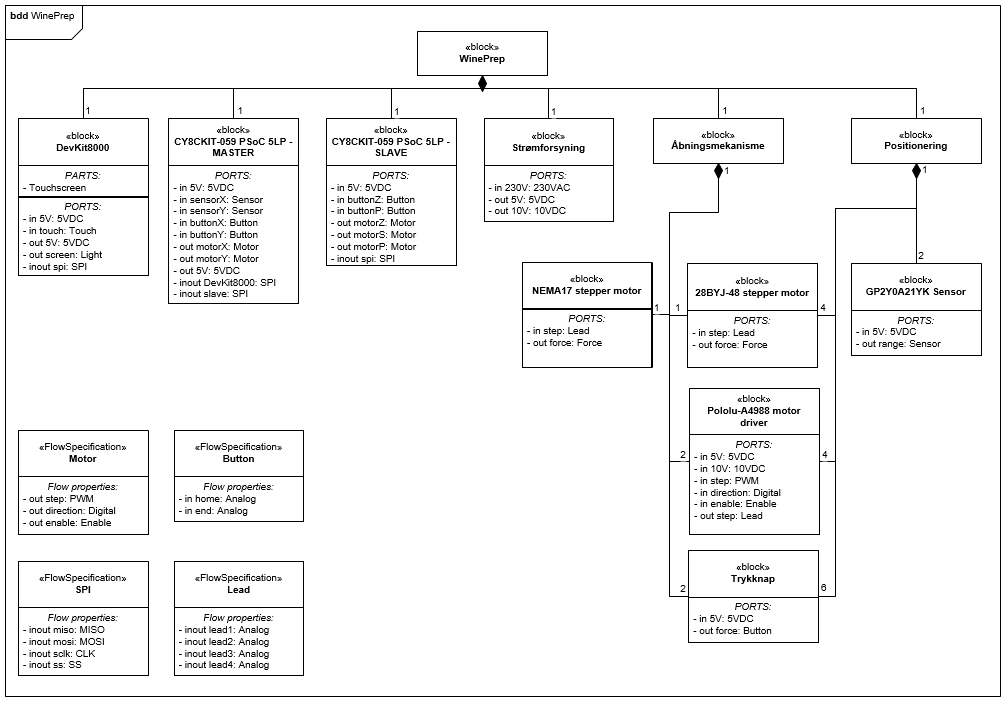
\includegraphics[scale=0.33]{tex/Arkitektur/Fotos/HW/BDD_winePrep}
\caption{BDD for WinePrep}
\end{figure}

Åbningsmekanisme:
Til selve åbningen af en vinflaske er der konstrueret en åbningsmekanisme. Den indeholder to motorer, en til iskruning, og en til optrækning.
For at kunne holde styr på skruens position, er der implementeret to trykknapper, der indikerer start og slut position. Motorene bliver styret via 
pololu motor drivere.   

Positionering:
For at detektere vinflaskens position og positionere åbningsmekanismen korrekt, anvendes en positioneringsmekanisme. Herpå er monteret to motorer som finder
vinflaskens x og y koordinator vha. sensorer. Z koordinatet bliver reguleret af yderligere to motorer, som hæver og sænker åbningsmekanismen. 
Der er implementeret to trykknapper, en som indikerer at åbningsmekanismen er tilstrækkelig tæt på vinflaskens åbning, den anden indikerer startpositionen. 
Yderligere fire trykknapper indikerer at x/y motorerne har nået deres yderposition. Alle motorene bliver ligeledes styret via pololu motor drivere.        
      
Devkit8000: 
Dette er et prototypekit, hvorpå Linux distribution ångström er installeret. Det er via devkittets touchskærm at interaktion med brugeren foregår. 
Denne enhed har dermed til opgave at tage imod input fra brugeren og sende disse videre i systemet, samt at give brugeren status beskeder. Den er forbundet til
PSoc Master via en SPI forbindelse.

PSoC Master:
PSoC er en programmerbar CPU enhed med GPIO pins, som har ansvaret for styring/aflæsning af hardware enheder. PSoC Master er forbundet til positionering, 
hvor den styrer x/y motorer via pololu motor drivere, og aflæser x/y sensorer samt x/y trykknapper. Den er forbundet med PSoC Slave via SPI.  

PSoC Slave:
Denne enhed styrer via pololu motor drivere de to z motorer på positionering, samt motorene på åbningsmekanismen. Den aflæser også z trykknapper på 
positionering og trykknapper på åbningsmekanismen.  

Strømforsyning:
Denne enhed leverer strøm til de enkelte hardware blokke. De tre CPU'er skal hver have 5 volt, det samme skal sensorer og trykknapper. Pololu motor driverne 
skal have både 5 og 10 volt.\\

\begin{figure}[H]
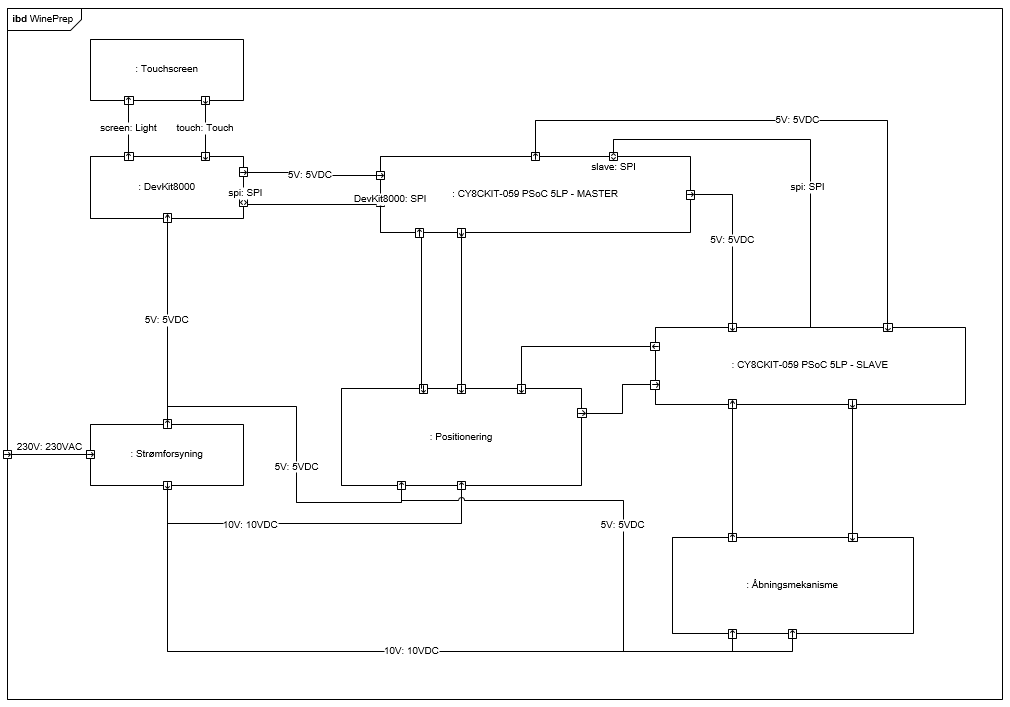
\includegraphics[scale=0.35]{tex/Arkitektur/Fotos/HW/IBD_winePrep}
\caption{\textbf{IBD for winePrep}}
\end{figure}


\section{Software}

Systemet indeholder som tidligere nævnt tre CPU'er, hvorpå der er allokeret software til interaktion med brugeren samt styring/aflæsning af diverse 
motorer, sensorer og trykknapper. I dette afsnit vil arkitekturen for systemets software blive beskrevet. \\

\begin{figure}[H]
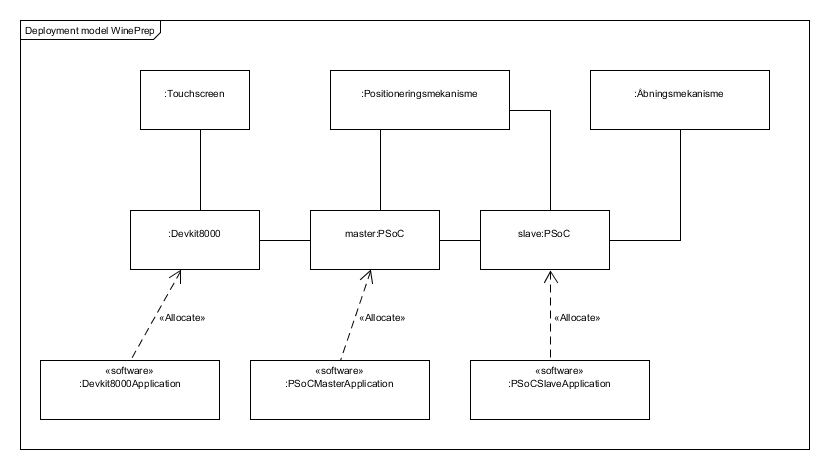
\includegraphics[scale=0.4]{tex/Arkitektur/Fotos/SW/Allokeringsdiagram}
\caption{Software allokeringsdiagram for winePrep}
\end{figure}  

\subsection{Devkit8000 (Linux platform)}

Devkit8000 har ansvaret for interaktion med brugeren via touchskærm. Derfor har systemet brug for en grafisk brugergrænseflade (GUI), hvorpå der er
implementeret virtuelle knapper, som gør det muligt at oversætte de fysiske tryk til kommandoer, der kan sendes videre i systemet. Der skal også kunne vises
status beskeder til brugeren, så denne er klar over systemets tilstand. Dette implementeres vha. viduer med tekstbeskeder. For at kunne sende brugerinputs 
videre i systemet skal devkittet forbindes til PSoC master via SPI. Da der køres med Linux på Devkit8000 kræves det derfor at en SPI device driver bliver
indsat i kernen. Devkit8000 har altså to boundary klasser, som viser grænsefladerne for devkittet. I klassediagramet ses også en protokolklasse for SPI, denne 
indeholder blot information til dekodning af de bits som bliver sendt over SPI.\\

\begin{figure}[H]
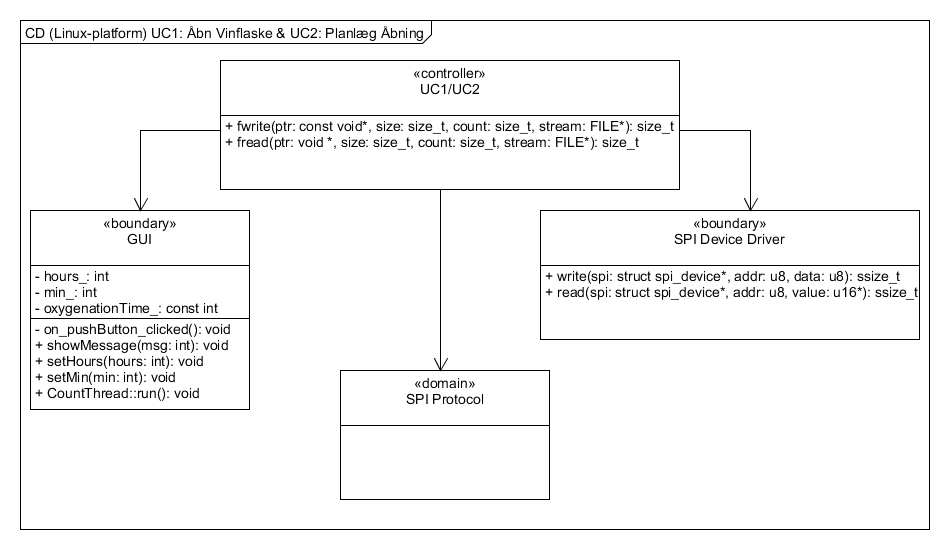
\includegraphics[scale=0.4]{tex/Arkitektur/Fotos/SW/Klassediagram_Linuxplatform}
\caption{Klassediagram Devkit8000}
\end{figure}

Med udgangpunkt i usecasen "åbn vinflaske", vil interaktionen mellem devkittet og boundaryklasserne blive beskrevet. 
GUI repræsenterer her grænsefladen til brugeren, og når denne trykker på en virtuel knap, kaldes write metoden fra controllerklassen, som skriver den korrekte 
kommando ud til SPI device driveren. Læsning fra SPI device driveren indledes også fra GUI, og når controller klassen har læst data, sendes status beskeder 
tilbage til GUI, og dermed informeres brugeren.\\

\begin{figure}[H]
\includegraphics[scale=0.4]{tex/Arkitektur/Fotos/SW/Sekvensdiagram_åbnvinflaske_Linuxplatform}
\caption{Sekvemdiagram for usecasen "Åbn vinflaske" på Devkit8000}
\end{figure}

\subsection{PSoC Master og PSoC slave}
PSoC Master og PSoC Slave vil blive beskrevet under samme afsnit da de deler klasse- og sekvensdiagrammer. 
Grunden til de ikke er opdelt er for overskueligehedens skyld. Da PSoC enhederne deler ansvaret for styring af positionering, giver det mening at de er 
indkluderet i samme sekvensdiagram. Det vil sige at der er to controllerklasser i klasse- og sekvensdiagrammerne. 

PSoC Master har to SPI boundary klasser, en til kommunikation med Devkit8000, og en til PSoC slave. Herudover er der boundary klasser til x/y motorer og 
sensorer på positionering. 
PSoC slave har SPI boundary klasse til kommunikation med PSoC Master og til z motorer på positionering, og motorer på åbningsmekanismen. Begge PSoC enheder har
en SPI protokol til dekodning af SPI kommandoer.\\

\begin{figure}[H]
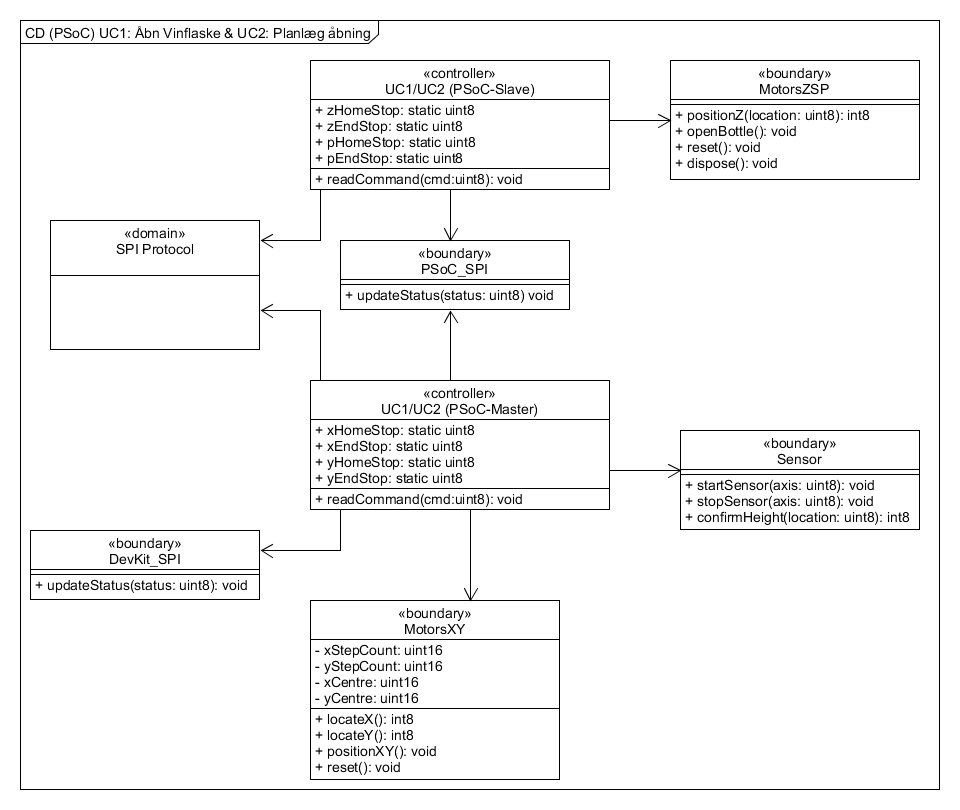
\includegraphics[scale=0.4]{tex/Arkitektur/Fotos/SW/Klassediagram_PSoC}
\caption{Klassediagram PSoC Master/Slave}
\end{figure}

Usecasene "åbn vinflaske" og "planlæg åbning" og samlet under det samme sekvensdiagram, da der fra PSoC enhedernes synspunkt sker det samme, nemlig 
åbning af en vinflaske. Timing af åbningen foregår på Devkit8000, og har ingen relevans for PSoC enhederne. Der er ikke medtaget alternative scenarier i 
sekvensdiagrammet, da disse er trivieller, og blot skaber unødvendig uoverskuelighed. Selve åbningen initieres fra SPI forbindelsen til Devkit8000. Herefter
sætter PSoC master x/y motorer til vha. sensorerne at finde flaskens x/y plasering. Når disse er fundet gives der besked til PSoC slave om at aktivere z motorene
og finde den rette afstand til flaskens top. Når denne er fundet påbegyndes åbningen af vinflasken, og derefter dispensering af proppen. Sekvensdiagrammet
afsluttes med en retur besked tilbage til Devkit8000 via SPI om succesfuld åbning.\\

\begin{figure}[H]
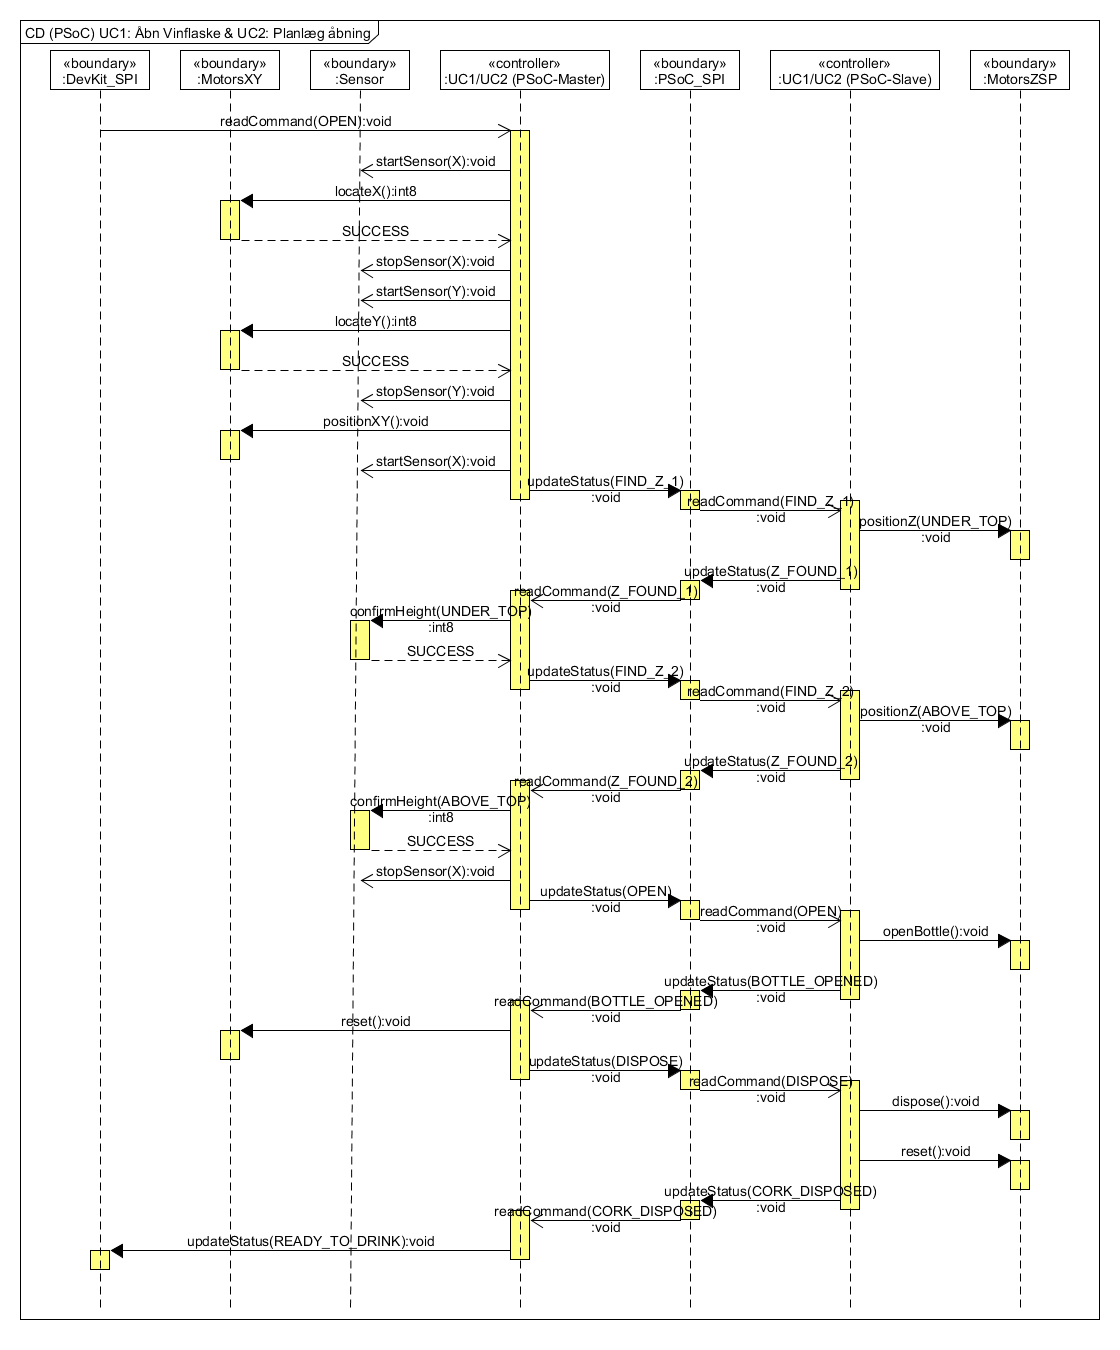
\includegraphics[scale=0.4]{tex/Arkitektur/Fotos/SW/Sekvendiagram_PSoC}
\caption{Sekvensdiagram for usecasene "åbn vinflaske" og "planlæg åbning" på PSoC Master/Slave}
\end{figure}

\section{Design}
\label{sec:Design}
\subsection{Positionering}
\label{sub:Pos}
Positionering består af 2 sensorer som drives af aktuatorer på de tre akser. Én motor på henholdsvis x og y flytter disse to akser mens to motorer driver z-aksen. \\
Som set i allokeringsdiagrammet\footnote{Figur \ref{Allokering_WinePrep} i kapitel \ref{sec:Arkitektur}} benyttes en PSoC til at styre disse motorer og sensorer. Det forudsættes, at der til at kontrollere, om bestemte punkter på akserne er nået, benyttes trykknapper. Når disse påtrykkes, igangsættes en interruptrutine på PSoC'ene.

\subsubsection{Hardware}
\label{pos_hw}
\myparagraph{Detektering}
At lokalisere flasken kræver en type af sensor. Embedded Stocks udvalg var begrænset så valget stod mellem to typer af afstandsmålere som enten vha. lys eller ultralyd kan detektere et objekt.
\\
\\
Tabel \ref{tab:Sensor_precision} viser forskellen i præcision for afstandsmåling mellem ultralydssensoren, HC-SR04, og  lasersensoren, GP2Y0A21YK\footnote{Se kapitlet Test afsnit om lasersensor}. Præcisionskravet er 1 mm for at \textbf{Åbningsmekanismen} har det mest centreret punkt på proppen at åbne.

\begin{table}[H]
	\centering
	\begin{tabular}{ |l|c| }
  		\hline
   		& Faktisk præcision \\
  		\hline 
  		HC-SR04 & 3 mm \\
  		\hline
  		GP2Y0A21YK  & 2,57 mm \\
  		\hline
	\end{tabular}
	\caption{De to sensores præcision}
	\label{tab:Sensor_precision}
\end{table}

\noindent
Tabellen udmundede i et fravalg af HC-SR04\footnote{Se \url{https://www.elextra.dk/main.aspx?page=article&artno=H16466}} sensoren fordi dennes præcision er mere unøjagtig. Da begge sensorer ikke opfylder kravet måtte en anden løsning om præcision findes. Denne kan ses under afsnittet om Aksestyring.
\\
\\
Sensorens (GP2Y0A21YK) ansvar er derfor kun at registrere om der er et objekt eller ej. Ved at sammenligne afstanden, målt i volt\footnote{Datablad for GP2Y0A21YK}, med et referencepunkt som er konstant\footnote{Dokumentation for Konstruktion} er det muligt at detektere for en flaske.
\\
\\
Fordi PSoC 5LP er valgt som microcontroller kan håndteringen af sensoren gøres i PSoC Creator. Det analoge signal fra sensoren konverteres til digitalt med SAR\_ADC komponenten\footnote{Datablad SAR\_ADC i bilagene}.

\myparagraph{Aksestyring}
Til at flytte akserne bruges motoren 28BYJ-48\footnote{Datablad for 28BYJ-48}. Valget er taget på baggrund af en analyse, udarbejdet ud fra kurserne GFV og EFYS, af forskellige typer af motorer, som viser at steppere generelt er DC- og servomotorer overlegne i præcision. En bevidsthed om at sensorerne ikke opfyldte præcisionskravet på 1 mm er også grundlaget for at vælge 28BYJ-48. Desuden udbyder Embedded Stock kun denne model, og ikke andre motorer, i et antal, som skal bruges i projektet.
\\
\\
I full-step mode flytter motoren aksen 0,04 mm\footnote{Se bilag Afstand per step for 28BYJ-48} per step, som er langt mere præcis end projektet kræver. Dermed er det ikke sensoren der afgør hvor flasken befinder sig, men motorerne. Dette gøres på softwaresiden som kan læses længere nede.
\\
\\
Valget af denne motor begrænser hastigheden hvormed akserne bliver flyttet fordi antallet af steps per rotation for skaftet er så stort.

\myparagraph{Unipolær motor}
28BYJ-48 er bygget som unipolær og kan styres sekventielt gennem fire transistorer\footnote{Dokumentation Unipolær motor}, hvilket ULN2003AN boardet\footnote{Datablad for ULN2003AN} kan bruges til. Et step tages ved at tilføre en transistor nok strøm til at den "åbner" og på den måde kan en strøm løbe i en af motorens spoler. I databladet for 28BYJ-48 ses en rød ledning der lader til at være sat på midterudtaget af de to spoler. Den røde ledning deler de to spoler i fire halve spoler. Ledningen fungerer som strømbærer til spolerne mens de fire andre ledninger skiftevis ledes til GND.
\\
\\
Momentet for motoren er dog relativt svagt, som kan ses under kapitlet Test, hvor den unipolære motor ikke har tilstrækkelig moment til at drive akserne uden små ophold. Udfordringen med motorens moment løses ved at ændre den til bipolær.

\myparagraph{Bipolær motor}
Med baggrund i Biot-Savarts lov er det udledt at B-feltet i en spole er proportional med antallet af viklinger i spolen, som ses i ligning \ref{eq:Biot_Savars}. For uddybning af denne udledning henvises til bilag\footnote{Se bilag Biot-Savarts lov}.

\begin{equation} \label{eq:Biot_Savars}
	B = \frac{\mu_0 \cdot i}{2 \cdot r} \cdot N
\end{equation}

\noindent
Hvis teorien fra Biot-Savarts lov overføres til 28BYJ-48 betyder det, at motoren burde få det dobbelte moment ved, at fjerne den røde lednings forbindelse til resten af motoren således, at motoren får to hele spoler i stedet for fire halve. Motoren burde så have den dobbelte længde spole og dermed antages spolen at have dobbelt så mange viklinger. I tabel \ref{tab:motor_moment}, i kapitlet Test, er det faktiske moment noteret, hvor det ses at momentet blev mere end fordoblet ved at omdanne 28BYJ-48 til bipolær.
\\
\\
Hver bipolær motor styres gennem to H-broer så det er muligt at vende strømmen, og dermed vende retningen på motoren. Det er først gjort gennem chippen L298\footnote{Datablad for L298} hvis datablad har været udgangspunkt for to designede og implementerede vero boards\footnote{Se bilag Printdesign\_L298} som blev udarbejdet. Figur \ref{fig:L298} viser de to H-broer som L298 indeholder.

\begin{figure}[H]
	\centerline{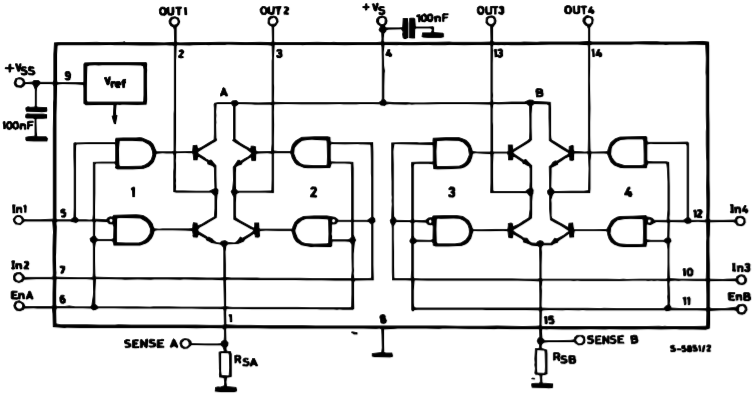
\includegraphics[scale=0.33]{tex/Design/L298}}
	\caption{L298 indeholdende to H-broer}
	\label{fig:L298}
\end{figure}

\noindent
Da boardsene aldrig kom til at fungere blev motor drivere af typen Pololu-A4988\footnote{Datablad for Pololu-A4988} taget i brug. Driveren følger samme princip som L298 med to H-broer, men motoren styres gennem et PWM-signal, en enable pin og en direction pin.
\subsection{Positionering}
\label{sub:Pos}
Positionering består af 2 sensorer som drives af aktuatorer på de tre akser. Én motor på henholdsvis x og y flytter disse to akser mens to motorer driver z-aksen. \\
Som set i allokeringsdiagrammet\footnote{Figur \ref{Allokering_WinePrep} i kapitel \ref{sec:Arkitektur}} benyttes en PSoC til at styre disse motorer og sensorer. Det forudsættes, at der til at kontrollere, om bestemte punkter på akserne er nået, benyttes trykknapper. Når disse påtrykkes, igangsættes en interruptrutine på PSoC'ene.

\subsubsection{Hardware}
\label{pos_hw}
\myparagraph{Detektering}
At lokalisere flasken kræver en type af sensor. Embedded Stocks udvalg var begrænset så valget stod mellem to typer af afstandsmålere som enten vha. lys eller ultralyd kan detektere et objekt.
\\
\\
Tabel \ref{tab:Sensor_precision} viser forskellen i præcision for afstandsmåling mellem ultralydssensoren, HC-SR04, og  lasersensoren, GP2Y0A21YK\footnote{Se kapitlet Test afsnit om lasersensor}. Præcisionskravet er 1 mm for at \textbf{Åbningsmekanismen} har det mest centreret punkt på proppen at åbne.

\begin{table}[H]
	\centering
	\begin{tabular}{ |l|c| }
  		\hline
   		& Faktisk præcision \\
  		\hline 
  		HC-SR04 & 3 mm \\
  		\hline
  		GP2Y0A21YK  & 2,57 mm \\
  		\hline
	\end{tabular}
	\caption{De to sensores præcision}
	\label{tab:Sensor_precision}
\end{table}

\noindent
Tabellen udmundede i et fravalg af HC-SR04\footnote{Se \url{https://www.elextra.dk/main.aspx?page=article&artno=H16466}} sensoren fordi dennes præcision er mere unøjagtig. Da begge sensorer ikke opfylder kravet måtte en anden løsning om præcision findes. Denne kan ses under afsnittet om Aksestyring.
\\
\\
Sensorens (GP2Y0A21YK) ansvar er derfor kun at registrere om der er et objekt eller ej. Ved at sammenligne afstanden, målt i volt\footnote{Datablad for GP2Y0A21YK}, med et referencepunkt som er konstant\footnote{Dokumentation for Konstruktion} er det muligt at detektere for en flaske.
\\
\\
Fordi PSoC 5LP er valgt som microcontroller kan håndteringen af sensoren gøres i PSoC Creator. Det analoge signal fra sensoren konverteres til digitalt med SAR\_ADC komponenten\footnote{Datablad SAR\_ADC i bilagene}.

\myparagraph{Aksestyring}
Til at flytte akserne bruges motoren 28BYJ-48\footnote{Datablad for 28BYJ-48}. Valget er taget på baggrund af en analyse, udarbejdet ud fra kurserne GFV og EFYS, af forskellige typer af motorer, som viser at steppere generelt er DC- og servomotorer overlegne i præcision. En bevidsthed om at sensorerne ikke opfyldte præcisionskravet på 1 mm er også grundlaget for at vælge 28BYJ-48. Desuden udbyder Embedded Stock kun denne model, og ikke andre motorer, i et antal, som skal bruges i projektet.
\\
\\
I full-step mode flytter motoren aksen 0,04 mm\footnote{Se bilag Afstand per step for 28BYJ-48} per step, som er langt mere præcis end projektet kræver. Dermed er det ikke sensoren der afgør hvor flasken befinder sig, men motorerne. Dette gøres på softwaresiden som kan læses længere nede.
\\
\\
Valget af denne motor begrænser hastigheden hvormed akserne bliver flyttet fordi antallet af steps per rotation for skaftet er så stort.

\myparagraph{Unipolær motor}
28BYJ-48 er bygget som unipolær og kan styres sekventielt gennem fire transistorer\footnote{Dokumentation Unipolær motor}, hvilket ULN2003AN boardet\footnote{Datablad for ULN2003AN} kan bruges til. Et step tages ved at tilføre en transistor nok strøm til at den "åbner" og på den måde kan en strøm løbe i en af motorens spoler. I databladet for 28BYJ-48 ses en rød ledning der lader til at være sat på midterudtaget af de to spoler. Den røde ledning deler de to spoler i fire halve spoler. Ledningen fungerer som strømbærer til spolerne mens de fire andre ledninger skiftevis ledes til GND.
\\
\\
Momentet for motoren er dog relativt svagt, som kan ses under kapitlet Test, hvor den unipolære motor ikke har tilstrækkelig moment til at drive akserne uden små ophold. Udfordringen med motorens moment løses ved at ændre den til bipolær.

\myparagraph{Bipolær motor}
Med baggrund i Biot-Savarts lov er det udledt at B-feltet i en spole er proportional med antallet af viklinger i spolen, som ses i ligning \ref{eq:Biot_Savars}. For uddybning af denne udledning henvises til bilag\footnote{Se bilag Biot-Savarts lov}.

\begin{equation} \label{eq:Biot_Savars}
	B = \frac{\mu_0 \cdot i}{2 \cdot r} \cdot N
\end{equation}

\noindent
Hvis teorien fra Biot-Savarts lov overføres til 28BYJ-48 betyder det, at motoren burde få det dobbelte moment ved, at fjerne den røde lednings forbindelse til resten af motoren således, at motoren får to hele spoler i stedet for fire halve. Motoren burde så have den dobbelte længde spole og dermed antages spolen at have dobbelt så mange viklinger. I tabel \ref{tab:motor_moment}, i kapitlet Test, er det faktiske moment noteret, hvor det ses at momentet blev mere end fordoblet ved at omdanne 28BYJ-48 til bipolær.
\\
\\
Hver bipolær motor styres gennem to H-broer så det er muligt at vende strømmen, og dermed vende retningen på motoren. Det er først gjort gennem chippen L298\footnote{Datablad for L298} hvis datablad har været udgangspunkt for to designede og implementerede vero boards\footnote{Se bilag Printdesign\_L298} som blev udarbejdet. Figur \ref{fig:L298} viser de to H-broer som L298 indeholder.

\begin{figure}[H]
	\centerline{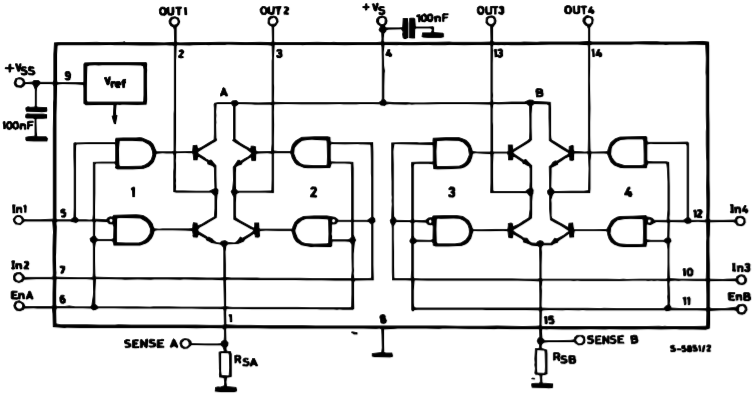
\includegraphics[scale=0.33]{tex/Design/L298}}
	\caption{L298 indeholdende to H-broer}
	\label{fig:L298}
\end{figure}

\noindent
Da boardsene aldrig kom til at fungere blev motor drivere af typen Pololu-A4988\footnote{Datablad for Pololu-A4988} taget i brug. Driveren følger samme princip som L298 med to H-broer, men motoren styres gennem et PWM-signal, en enable pin og en direction pin.
\subsection{Åbningsmekanisme}
\subsubsection{Hardware}
\myparagraph{Iskruning}
Ved at teste hvor stor en kraft der skal til for, at skrue proptrækkeren i proppen, kunne en aktuator vælges ud fra testen. Desværre for projektet har det været umuligt at finde ordentligt måleudstyr. Desuden har det ikke været muligt at sammenligne med lignende eksisterende produkter så et design af iskruning er aldrig opnået.

\myparagraph{Proptrækning}
Test af proptrækning med kraftmåler lånt fra Navitas giver et krav til motoren om moment på +25 kg\footnote{Se bilag Test_af_proptræk}. Ud fra kravet kunne kun en motor, en gearet NEMA17 som styres bipolært ligesom resten af motorerne, fra ASE benyttes til formålet. 
\subsection{Åbningsmekanisme}
\subsubsection{Hardware}
\myparagraph{Iskruning}
Ved at teste hvor stor en kraft der skal til for, at skrue proptrækkeren i proppen, kunne en aktuator vælges ud fra testen. Desværre for projektet har det været umuligt at finde ordentligt måleudstyr. Desuden har det ikke været muligt at sammenligne med lignende eksisterende produkter så et design af iskruning er aldrig opnået.

\myparagraph{Proptrækning}
Test af proptrækning med kraftmåler lånt fra Navitas giver et krav til motoren om moment på +25 kg\footnote{Se bilag Test_af_proptræk}. Ud fra kravet kunne kun en motor, en gearet NEMA17 som styres bipolært ligesom resten af motorerne, fra ASE benyttes til formålet. 
\subsubsection{Seriel kommunikation}

\textbf{Devkit8000-PSoC Master:} \\

Som beskrevet i analysen for SPI (reference), blev denne protokol valgt pga. den kendskab gruppen allerede havde fra HAL øvelse 6 (reference). 
SPI device driveren fra denne øvelse blev benyttet som udgangspunkt til at lave en tilpasset driver, som kunne kommunikere med PSoC Master. 
Denne forbindelse viste sig dog at volde store problemer for gruppen, og det lykkedes ikke at få hverken sendt eller modtaget data med denne driver.\\

Det blev herefter besluttes at der ikke skulle bruges mere tid på selv at lave en driver, og istedet benytte en SPI device driver som var udleveret fra skolen.
Dog var det blot den binære fil som var tilgængelig, hvilket betød at der ikke var adgang til source-koden. Dette gjorde at gruppen ikke kunne tilpasse driveren,
og alt information omkring opsætningen for SPI forbindelse måtte udledes fra det PSoC-Creator program som medfulgte. 

\begin{figure}[H]
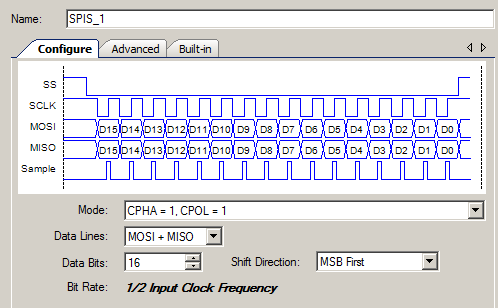
\includegraphics[scale=0.6]{tex/Design/SPI/Clock_mode_SPI}
\caption{Opsætning for SPI forbindelse Devkit8000-PSoC Master}
\end{figure}

Ud fra figur xx, kan det aflæses at SPI clock mode er sat til CPHA = 1 og CPOL = 1, og bitsperword til 16 databits. Det PSoC program som var udleveret blev brugt
som skabelon for gruppens eget program til PSoC master, dog med nogle modifikationer. Især behandlingen af de databits som blev modtaget fra devkittet blev 
genbrugt, da der ikke kunne ændres på disse bits. Koden består dybest set at en interrupt service rutine (ISR), som kaldes hver gang
der modtages data fra devkittet. I ISR er der implementeret en switch, der sørger for at de rigtige metoder kaldes alt efter hvilke databits der modtages.
For mere information omkring koden for PSoC master henvises til bilag(navn på bilag). \\

\textbf{PSoC Master - PSoC Slave:} \\

Til SPI forbindelsen mellem PSoC Master og PSoc slave havde gruppen frie hænder til opsætte SPI. Her blev clock mode valgt til CHPA = 0 og CPOL = 0, og 
bitsperword til 8. Grunden til der kun bliver sendt 8 bits her, er at det er tilstrækkeligt til den simple form for kommunikation der er mellem PSoc enhederne.
8 databits ville også have været fint for Devkit-PSoC forbindelsen, men som tidligere nævnt kunne det ikke ændres da der ikke var adgang til SPI device driveren
på Devkit8000. Clock mode er ændret til default værdien fra PSoC-Creator, og har ikke nogen betydning for kommunikationen så længe begge PSoC enheder har samme
clock mode. Koden for PSoC Slave indeholder ligesom i PSoC master en switch der alt efter de modtagne databits kalder metoder til udførsel af diverse opgaver. 
For mere information omkring koden for PSoC slave henvises til bilag(navn på bilag).   



\subsubsection{GUI}

Da programmet QT blev anvendt til at designe og implementer brugergrænsefladen. Udfordringerne bestod primært i at kendskabet til programmet QT ikke var særligt stort. Da QT selv skaber klasserne og metoderne er det svært at beskrive disse på forhånd. Derfor blev det besluttet at klasserne først skulle udarbejdes efter at brugergrænsefladen var designet. 

For at holde styr på den indtastede og den resterende tid er der blev oprettet en Count klasse . Denne count klasse er implementeret som en domainklasse da det er her den resterende tid for vinåbningen gemmes. Det er denne klasse som skal sørge for at tiden tælles ned når den startes. Illustrationen af countklassen kan ses på figur \ref{CT_CD}.

\begin{figure}[H]
	\centerline{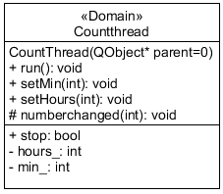
\includegraphics[scale=1]{tex/Design/GUI/Fotos/CountThread}}
	\caption{CountThread klasse illustreret}
	\label{CT_CD}
\end{figure}

Der er i alt 2 klasser i brugergrænsefladen. Der er en klasse for MainWindow, hvor alle funktionerne er defineret. MainWindow er klassen som sørger for at vise den grafiske brugergrænseflade. Det er her alle trykknap funktionerne er defineret. Klassen ses illustreret på figur \ref{MW_CD}. 

\begin{figure}[H]
	\centerline{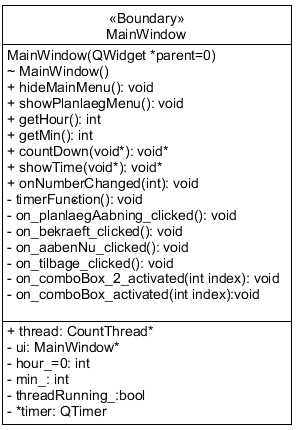
\includegraphics[scale=1]{tex/Design/GUI/Fotos/MainWindow}}
	\caption{MainWindow klasse illustreret}
	\label{MW_CD}
\end{figure}

Brugergrænsefladen er state styret. Derfor har det været nødvendigt at lave et statemachine diagram for brugergrænsefladen. Der er i alt 3 overordnede states for hele system. De tre states er, ”Åbning”, ”Venter på åbning” og ”Åbning stoppet”.

Når vinåbneren er i gang med at åbne en vinflaske, så er den i staten ”Åbning”. Der er to ting der kan bringe systemet til denne state. Den første er at brugeren igennem brugergrænsefladen trykker på knappen ”Åbn nu”. Dette vil få systemet til at starte åbningen, og dermed bringe systemet i staten ”Åbning”. Den anden handling der kan bringe systemet i denne state, er når tiden under ”Planlæg åbning” menuen udløber og systemet dermed starter åbningen på vinflasken. 

Staten ”Venter på åbning” startes ved at brugeren under ”Planlæg åbning” menuen sætter en tid og trykker på bekræft. Når brugeren starter tiden, vil systemet begynde at tælle ned indtil åbningen påbegyndes. Den tid hvor systemet venter på at tiden udløber således at åbningen kan påbegyndes er staten ”Venter på åbning”.

Den sidste state er ”Åbning stoppet”. Det er denne state systemet starter ud med at være i. I denne state foretager systemet sig ingenting. Når åbningen er færdiggjort kommer systemet i denne state.
\section{Implementering}
\chapter{Implementering}
\section{Hardware}
\label{HW_Implementering}
På figur \ref{fig:Pololu-A4988} ses hvordan Pololu-A4988 opsættes til PSoC 5LP og en motor. I den endelige impementering er antallet af Pololu-A4988 motor drivere og motorer i forholdet 1:1. Driveren fungerer som bindeled mellem PSoC 5LP og motoren. Tabel \ref{tab:Pololu-A4988_pin_configuration} viser pin konfigureringen fra Pololu-A4988 til henholdsvis PSoC 5LP og 28BYJ-48. Rækkefølgen af pins i tabellen svarer til billedet fra figur \ref{fig:Pololu-A4988} læst fra øverste venstre hjørne. MS1, MS2 og MS3 er ikke forbundet til noget. RESET og SLEEP er forbundet til hinanden.

\begin{figure}[H]
	\centerline{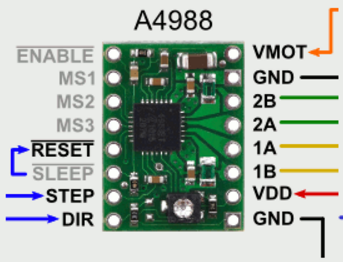
\includegraphics[scale=0.6]{Pololu-A4988.png}}
	\caption[]{Pololu-A4988}\footnotemark
	\label{fig:Pololu-A4988}
\end{figure}
\footnotetext{https://forum.pololu.com/t/a4988-issue/6518}

\begin{table}[H]
  \centering
\begin{tabular}{ |l|c|c|c| }
  \hline
   & \textbf{PSoC 5LP} & \textbf{Motor} & \textbf{VDD} \\
  \hline 
  ENABLE & X & & \\
  \hline
  STEP & X & & \\
  \hline
  DIR & X & & \\
  \hline
  VMOT (10V) & & & X \\
  \hline
  GND & X & & X \\
  \hline
  2B & & X & \\
  \hline
  2A & & X & \\
  \hline
  1A & & X & \\
  \hline
  1B & & X & \\
  \hline
  VDD (5V) & & & X \\
  \hline
  GND & & & X \\
  \hline
\end{tabular}
\caption{Pololu-A4988 pin konfigurering}\label{tab:Pololu-A4988_pin_configuration}
\end{table}

\noindent
VDD er altså spændingsforsyning som leverer både 5V og 10V til henholdsvis driveren og motoren.
\\
\\
Sensorerne har tre pins som alle er sat direkte til PSoC 5LP Master, som vist i tabel \ref{tab:Sensor_pin_konfigurering}.

\begin{table}[H]
  \centering
\begin{tabular}{ |l|c| }
  \hline
  \textbf{GP2Y0A21YK Sensor} & \textbf{PSoC 5LP}\\
  \hline 
  $V_0$ & P[X:X] \\
  \hline 
  GND & P[X:X] \\
  \hline 
  $V_CC$ & P[X:X] \\
  \hline 
\end{tabular}
\caption{GP2Y0A21YK sensor implementeret med PSoC 5LP}\label{tab:Sensor_pin_konfigurering}
\end{table}
\subsection{Software}
\subsubsection{PSoC}
Klasserne fra klassediagrammet blev implementeret i form af hver deres headerfil efter princippet om høj samhørighed - lav kobling. \textit{main}-funktionen blev formet som en state-machine, der vha. en switch påkaldte de metoder, der skulle udføres på et givent tidspunkt i eksekveringen af programmet i henhold til sekvensdiagrammet(reference!!!!). Disse switches' cases bestemtes ud fra de kommandoer/beskeder, de enkelte PSoC's modtog fra hinanden eller DevKit8000. Der er ligeledes blevet oprettet en seperat \textit{status}-fil, som indeholder adskillige kommandoer/beskeder og forkortelser, der bruges igennem programmet, for at holde koden overskuelig og øge læsbarheden af denne.

\myparagraph{Hardware-grænseflade}
\mysubparagraph{Sensorer}
Til at måle sensorerne benyttedes en SAR-ADC, som, efter hvert sample, returnerede en værdi i \textit{counts}. For at sammenligne med (GRAF FRA SENSOR-DATABLAD) konverteredes disse værdier til mV. Dermed kunne der fastslås, hvor vidt en flaske var registreret, ud fra afstanden forbundet med den målte spænding.

\mysubparagraph{Motorer}
Motorerne styredes vha. et PWM-signal, som gik fra en given GPIO-pen ud til STEP-inputtet på A4988-driveren, som talte et step op for hver rising edge på PWM-signalet, samt to digitale signaler, der gik til henholdsvis ENABLE- og DIRECTION-inputtene på driveren.

\mysubparagraph{Knapper}
Knapperne implementeredes som interrupts der trigger på rising edge. Disse var hovedårsagen til, at der skulle min. 2 PSoS's, da hvert interrupt optager en port på PSoC'en, som kun har 6 til rådighed, mens der var behov for 8.
\subsubsection{Seriel kommunikation}

\textbf{Devkit8000-PSoC Master:} \\

Som beskrevet i analysen for SPI (reference), blev denne protokol valgt pga. den kendskab gruppen allerede havde fra HAL øvelse 6 (reference). 
SPI device driveren fra denne øvelse blev benyttet som udgangspunkt til at lave en tilpasset driver, som kunne kommunikere med PSoC Master. 
Denne forbindelse viste sig dog at volde store problemer for gruppen, og det lykkedes ikke at få hverken sendt eller modtaget data med denne driver.\\

Det blev herefter besluttes at der ikke skulle bruges mere tid på selv at lave en driver, og istedet benytte en SPI device driver som var udleveret fra skolen.
Dog var det blot den binære fil som var tilgængelig, hvilket betød at der ikke var adgang til source-koden. Dette gjorde at gruppen ikke kunne tilpasse driveren,
og alt information omkring opsætningen for SPI forbindelse måtte udledes fra det PSoC-Creator program som medfulgte. 

\begin{figure}[H]
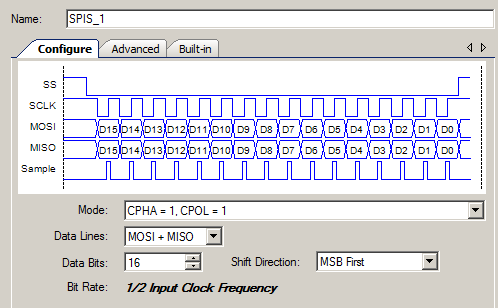
\includegraphics[scale=0.6]{tex/Design/SPI/Clock_mode_SPI}
\caption{Opsætning for SPI forbindelse Devkit8000-PSoC Master}
\end{figure}

Ud fra figur xx, kan det aflæses at SPI clock mode er sat til CPHA = 1 og CPOL = 1, og bitsperword til 16 databits. Det PSoC program som var udleveret blev brugt
som skabelon for gruppens eget program til PSoC master, dog med nogle modifikationer. Især behandlingen af de databits som blev modtaget fra devkittet blev 
genbrugt, da der ikke kunne ændres på disse bits. Koden består dybest set at en interrupt service rutine (ISR), som kaldes hver gang
der modtages data fra devkittet. I ISR er der implementeret en switch, der sørger for at de rigtige metoder kaldes alt efter hvilke databits der modtages.
For mere information omkring koden for PSoC master henvises til bilag(navn på bilag). \\

\textbf{PSoC Master - PSoC Slave:} \\

Til SPI forbindelsen mellem PSoC Master og PSoc slave havde gruppen frie hænder til opsætte SPI. Her blev clock mode valgt til CHPA = 0 og CPOL = 0, og 
bitsperword til 8. Grunden til der kun bliver sendt 8 bits her, er at det er tilstrækkeligt til den simple form for kommunikation der er mellem PSoc enhederne.
8 databits ville også have været fint for Devkit-PSoC forbindelsen, men som tidligere nævnt kunne det ikke ændres da der ikke var adgang til SPI device driveren
på Devkit8000. Clock mode er ændret til default værdien fra PSoC-Creator, og har ikke nogen betydning for kommunikationen så længe begge PSoC enheder har samme
clock mode. Koden for PSoC Slave indeholder ligesom i PSoC master en switch der alt efter de modtagne databits kalder metoder til udførsel af diverse opgaver. 
For mere information omkring koden for PSoC slave henvises til bilag(navn på bilag).   



\subsubsection{GUI}

Da brugergrænsefladen skulle laves, var der ingen tvivl om hvilket program der skulle anvendes til udarbejdelse af brugergrænsefladen. Programmet QT blev valgt da der tidligere har været arbejdet med QT i forbindelse med andre semesterprojekter. QT er et program som giver en masse muligheder som kan udnyttes. For eksempel giver QT en drag and drop mulighed, således at brugergrænsefladens udseende kan designes på en meget let og brugervenlig måde.
Sproget som brugergrænsefladen er skrevet i er C++ da det er dette sprog som teamet har haft størst erfaring med.

For at kommunikere med SPI driveren som ligger på Devkit8000 er funktionerne fread() og fwrite() brugt. Et eksempel på hvordan funktionen fwrite() blev brugt kan ses på figur x.

\begin{figure}[H]
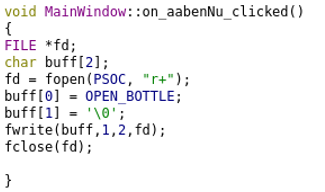
\includegraphics[scale=1]{tex/Implementering/GUI/GUI-implementering/Billeder/kodeeksempel.png}
\caption{Åben nu funktionen implementerets}
\end{figure}

På figuren ses det hvordan funktionen for trykknappen ”Åbn nu” er implementeret. PSOC er tidligere i koden blevet defineret som path’en på PSoC driven. I koden kan man se at OPEN\_BOTTLE, skrives til PSoC driveren ved hjælp af fwrite(). OPEN\_BOTTLE er tidligere blevet defineret som 5, hvilket i SPI protokollen betyder at vinen skal åbnes. Det er samme kode der bruges til funktionen ”Planlæg åbning”.
For at få tiden talt ned og samtidigt displayet på skærmen er der blevet benyttet threads. Implementeringen af dette kan ses i dokumentationsbilaget x.

\section{Test}
\subsection{Motorer og sensorer}
Test af motorer og sensorer er foretaget med både uni- og bipolære motorer som er foregået efter samme metode, hvor komponenterne er testet enkeltvis og i moduler. Der er ikke foretaget modultest af motorer for iskruning af proptrækker eller proptræk fordi åbningsmekanismen aldrig blev færdig. Der er derfor kun foretaget modultest af akserne, dog i 2 omgange, hvor unipolære motorer senere blev udskiftet med bipolære.
\\
\\
Der er bygget et stativ til at teste forskellen i moment for uni- og bipolær som ses på figur \ref{fig:HW_stativ_test}.

\begin{figure}[H]
	\centerline{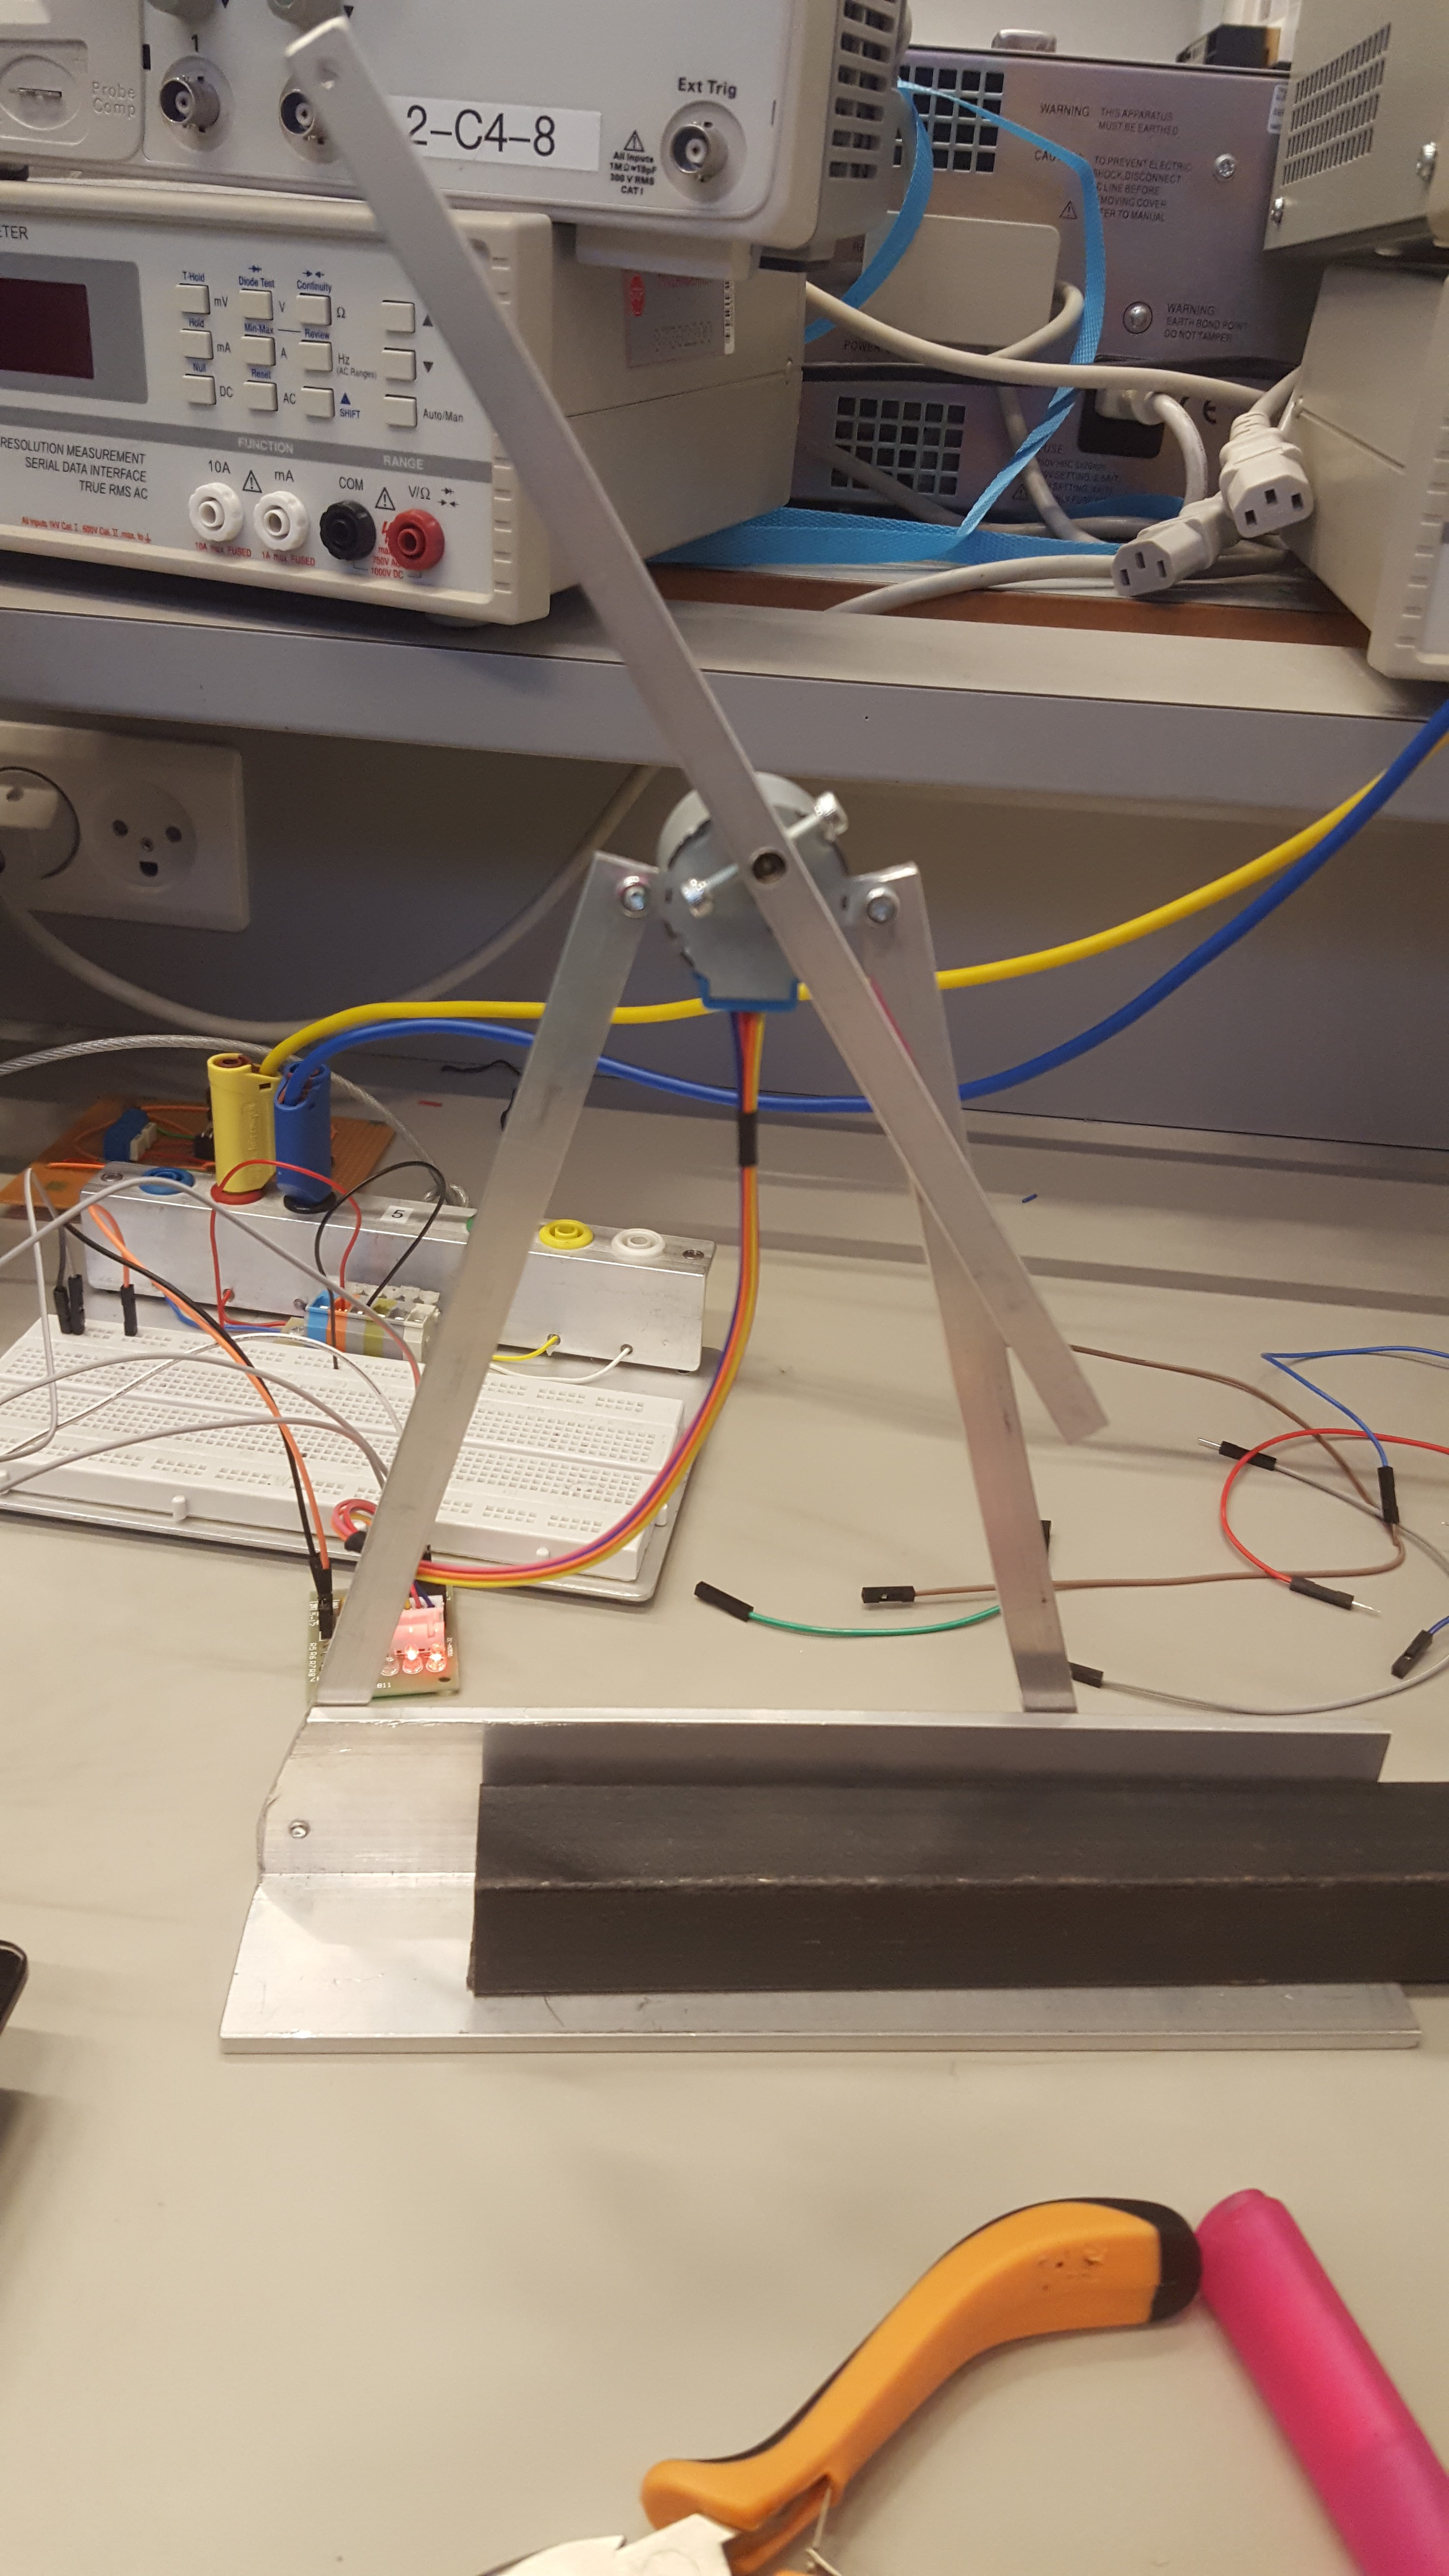
\includegraphics[scale=0.33]{HW_stativ_test.png}}
	\caption{Stativ til test af uni- og bipolær}
	\label{fig:HW_stativ_test}
\end{figure}
\subsubsection{Seriel kommunikation}

\textbf{Devkit8000-PSoC Master:} \\

Som beskrevet i analysen for SPI (reference), blev denne protokol valgt pga. den kendskab gruppen allerede havde fra HAL øvelse 6 (reference). 
SPI device driveren fra denne øvelse blev benyttet som udgangspunkt til at lave en tilpasset driver, som kunne kommunikere med PSoC Master. 
Denne forbindelse viste sig dog at volde store problemer for gruppen, og det lykkedes ikke at få hverken sendt eller modtaget data med denne driver.\\

Det blev herefter besluttes at der ikke skulle bruges mere tid på selv at lave en driver, og istedet benytte en SPI device driver som var udleveret fra skolen.
Dog var det blot den binære fil som var tilgængelig, hvilket betød at der ikke var adgang til source-koden. Dette gjorde at gruppen ikke kunne tilpasse driveren,
og alt information omkring opsætningen for SPI forbindelse måtte udledes fra det PSoC-Creator program som medfulgte. 

\begin{figure}[H]
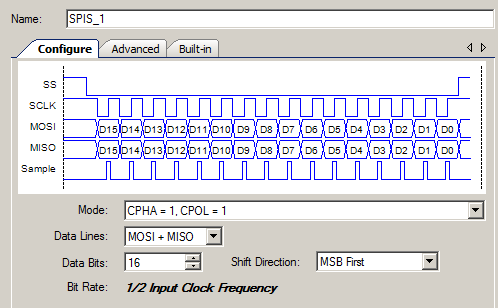
\includegraphics[scale=0.6]{tex/Design/SPI/Clock_mode_SPI}
\caption{Opsætning for SPI forbindelse Devkit8000-PSoC Master}
\end{figure}

Ud fra figur xx, kan det aflæses at SPI clock mode er sat til CPHA = 1 og CPOL = 1, og bitsperword til 16 databits. Det PSoC program som var udleveret blev brugt
som skabelon for gruppens eget program til PSoC master, dog med nogle modifikationer. Især behandlingen af de databits som blev modtaget fra devkittet blev 
genbrugt, da der ikke kunne ændres på disse bits. Koden består dybest set at en interrupt service rutine (ISR), som kaldes hver gang
der modtages data fra devkittet. I ISR er der implementeret en switch, der sørger for at de rigtige metoder kaldes alt efter hvilke databits der modtages.
For mere information omkring koden for PSoC master henvises til bilag(navn på bilag). \\

\textbf{PSoC Master - PSoC Slave:} \\

Til SPI forbindelsen mellem PSoC Master og PSoc slave havde gruppen frie hænder til opsætte SPI. Her blev clock mode valgt til CHPA = 0 og CPOL = 0, og 
bitsperword til 8. Grunden til der kun bliver sendt 8 bits her, er at det er tilstrækkeligt til den simple form for kommunikation der er mellem PSoc enhederne.
8 databits ville også have været fint for Devkit-PSoC forbindelsen, men som tidligere nævnt kunne det ikke ændres da der ikke var adgang til SPI device driveren
på Devkit8000. Clock mode er ændret til default værdien fra PSoC-Creator, og har ikke nogen betydning for kommunikationen så længe begge PSoC enheder har samme
clock mode. Koden for PSoC Slave indeholder ligesom i PSoC master en switch der alt efter de modtagne databits kalder metoder til udførsel af diverse opgaver. 
For mere information omkring koden for PSoC slave henvises til bilag(navn på bilag).   



\section{Test - GUI}

Det vigtigste der skulle testes ved brugergrænsefladen var at den kunne sende en hvilken som helst kommando ved hjælp af SPI driveren. Dette blev testet ved at forbinde Analog Discovery til Devkit8000’s SPI ben. Derefter blev funktionen Logic Analyzer benyttet til at måle på outputtet. Det var vigtigt at vide hvornår kommandoen blev sendt ud. Da touchfunktionen ikke har været optimal på Devkit8000 blev funktion ”Planlæg åbning” brugt til at teste hvad outputtet fra Devkit8000 var efter nedtællingen. Grunden til at funktionen ”Åbn nu” ikke blev brugt, var fordi at man skulle trykke mange gange på touchskærmen for at Devkittet ville reagere. Dette bragte en uønsket usikkerhed i testen. Derfor var det mere hensigtsmæssigt at teste med funktionen ”Planlæg åbning da man her kan se hvornår tiden udløber, og dermed hvornår der bør sendes en kommando ud. På figur x, kan det ses hvordan, det var muligt at sende kommandoen 5 ved at bruge ”Planlæg åbning” funktionen. 

\includegraphics{Billeder/test_GUI}
\caption{Åben nu funktionen implementerets}

\section{Resultater}
\subsection{Motor-/sensorstyring}
\subsubsection{Akserne}
Figur \ref{Bipolar} viser test opstillingen af bipolær motor på x-/y-akse, som validerede det forventede resultat, hvor aksen blev flyttet vha. det forøgede moment fra motoren. \\

\begin{figure}[H]
	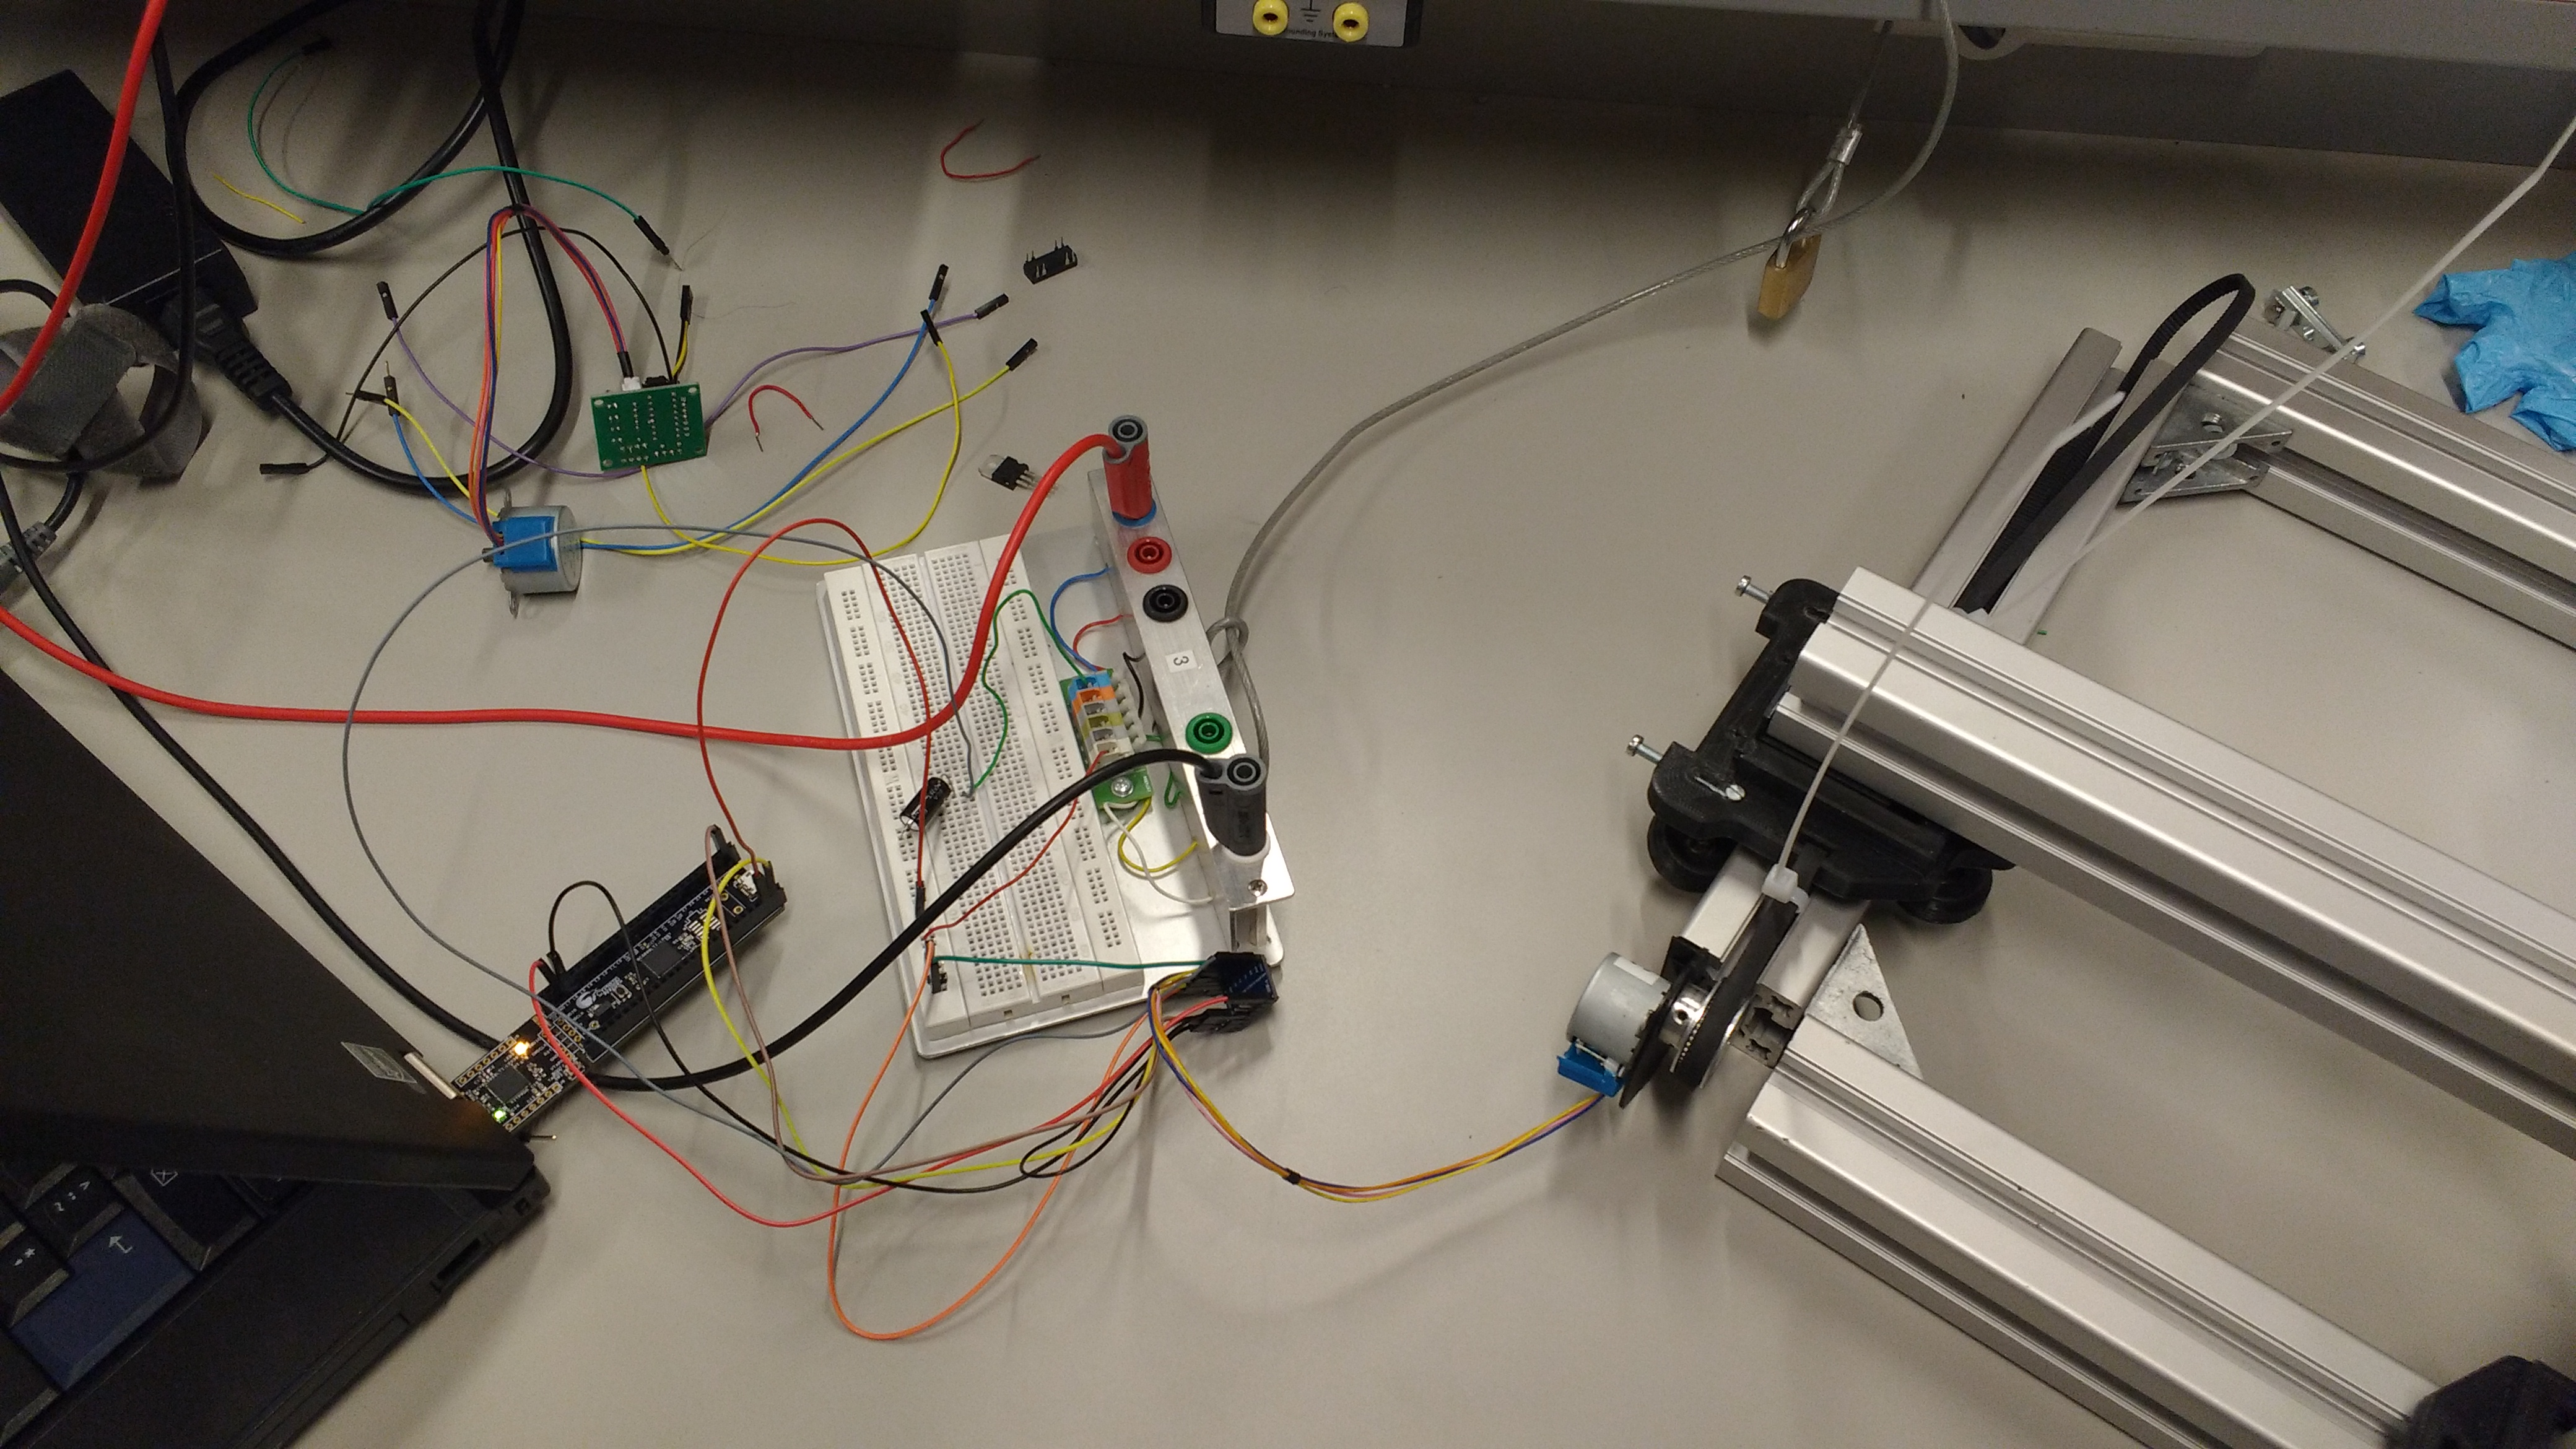
\includegraphics[scale=0.09]{tex/Test/Motor-sensor/Bipolar_test_opstilling.jpg}
	\caption{Test af bipolær motor på x-/y-akse}
	\label{Bipolar}
\end{figure}

Resultaterne fra testen, og andre lignende test af z-aksen (se evt. bilag xx), betød at en udvidet modultest kunne udføres hvori akserne samt detektering foregik. Desværre lykkedes det aldrig at få glidende bevægelser på akserne, som med stor sandsynlighed skyldes konstruktionens ujævnheder. \\

Sensorerne blev testet ved at lade forskellige materialer blive detekteret på afstand af varierende størrelser, hvor det viste sig at sensorerne var ret pålidelige når resultaterne blev holdt op mod Figur 4 i databladet (reference) for dem. Et resultat, målt i mV, kan ses på Figur \ref{Sensor_10cm} under fanebladet Value, ellers henvises til bilag xx for flere resultater. \\

\begin{figure}[H]
	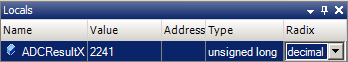
\includegraphics[scale=1]{tex/Test/Motor-sensor/Sensor_10cm.png}
	\caption{Resultat af detektering fra sensor ved 10 cm}
	\label{Sensor_10cm}
\end{figure}

Værdien for detektering ved 10 cm var 2241 mV som lægger sig tæt op ad de ca. 2300 mV der kan udledes af databladet, altså en afvigelse på 2,57\%, eller en unøjagtighed på 2,57 mm ved denne afstand. Sensorernes unøjagtighed ville altså være for stor ift. at en åbningsmekanisme skulle lægge sig over flasken og åbne den.
\subsubsection{Seriel kommunikation}

\textbf{Devkit8000-PSoC Master:} \\

Som beskrevet i analysen for SPI (reference), blev denne protokol valgt pga. den kendskab gruppen allerede havde fra HAL øvelse 6 (reference). 
SPI device driveren fra denne øvelse blev benyttet som udgangspunkt til at lave en tilpasset driver, som kunne kommunikere med PSoC Master. 
Denne forbindelse viste sig dog at volde store problemer for gruppen, og det lykkedes ikke at få hverken sendt eller modtaget data med denne driver.\\

Det blev herefter besluttes at der ikke skulle bruges mere tid på selv at lave en driver, og istedet benytte en SPI device driver som var udleveret fra skolen.
Dog var det blot den binære fil som var tilgængelig, hvilket betød at der ikke var adgang til source-koden. Dette gjorde at gruppen ikke kunne tilpasse driveren,
og alt information omkring opsætningen for SPI forbindelse måtte udledes fra det PSoC-Creator program som medfulgte. 

\begin{figure}[H]
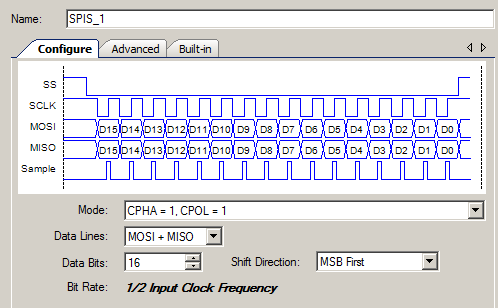
\includegraphics[scale=0.6]{tex/Design/SPI/Clock_mode_SPI}
\caption{Opsætning for SPI forbindelse Devkit8000-PSoC Master}
\end{figure}

Ud fra figur xx, kan det aflæses at SPI clock mode er sat til CPHA = 1 og CPOL = 1, og bitsperword til 16 databits. Det PSoC program som var udleveret blev brugt
som skabelon for gruppens eget program til PSoC master, dog med nogle modifikationer. Især behandlingen af de databits som blev modtaget fra devkittet blev 
genbrugt, da der ikke kunne ændres på disse bits. Koden består dybest set at en interrupt service rutine (ISR), som kaldes hver gang
der modtages data fra devkittet. I ISR er der implementeret en switch, der sørger for at de rigtige metoder kaldes alt efter hvilke databits der modtages.
For mere information omkring koden for PSoC master henvises til bilag(navn på bilag). \\

\textbf{PSoC Master - PSoC Slave:} \\

Til SPI forbindelsen mellem PSoC Master og PSoc slave havde gruppen frie hænder til opsætte SPI. Her blev clock mode valgt til CHPA = 0 og CPOL = 0, og 
bitsperword til 8. Grunden til der kun bliver sendt 8 bits her, er at det er tilstrækkeligt til den simple form for kommunikation der er mellem PSoc enhederne.
8 databits ville også have været fint for Devkit-PSoC forbindelsen, men som tidligere nævnt kunne det ikke ændres da der ikke var adgang til SPI device driveren
på Devkit8000. Clock mode er ændret til default værdien fra PSoC-Creator, og har ikke nogen betydning for kommunikationen så længe begge PSoC enheder har samme
clock mode. Koden for PSoC Slave indeholder ligesom i PSoC master en switch der alt efter de modtagne databits kalder metoder til udførsel af diverse opgaver. 
For mere information omkring koden for PSoC slave henvises til bilag(navn på bilag).   



\section{Diskussion af resultater}
\chapter{Diskussion af resultater}
\section{Motorer og sensorer}
\label{sec:HW_diskussion}
Den interessante test for motorer er den der viser forskellen i moment for uni- og bipolær motor. Ifølge Biot-Savarts lov burde den bipolære motor have forøget momentet med to gange, men resultatet viser sig at være betydeligt bedre. Det er svært at argumentere for om der er en eller flere årsager til resultatet, og hvad grunden til resultatet skyldes. Det kan dog konkluderes at der er flere faktorer der spiller ind ift. motorens moment, som ikke blev taget med i overvejelserne fordi databladet for 28BYJ-48 er mangelfuldt\footnote{Datablad 28BYJ-48}. Overvejelser omkring faktorerne kan ses i dokumentationen for bipolære motorer.
\\
\\

\subsubsection{Seriel kommunikation}

\textbf{Devkit8000-PSoC Master:} \\

Som beskrevet i analysen for SPI (reference), blev denne protokol valgt pga. den kendskab gruppen allerede havde fra HAL øvelse 6 (reference). 
SPI device driveren fra denne øvelse blev benyttet som udgangspunkt til at lave en tilpasset driver, som kunne kommunikere med PSoC Master. 
Denne forbindelse viste sig dog at volde store problemer for gruppen, og det lykkedes ikke at få hverken sendt eller modtaget data med denne driver.\\

Det blev herefter besluttes at der ikke skulle bruges mere tid på selv at lave en driver, og istedet benytte en SPI device driver som var udleveret fra skolen.
Dog var det blot den binære fil som var tilgængelig, hvilket betød at der ikke var adgang til source-koden. Dette gjorde at gruppen ikke kunne tilpasse driveren,
og alt information omkring opsætningen for SPI forbindelse måtte udledes fra det PSoC-Creator program som medfulgte. 

\begin{figure}[H]
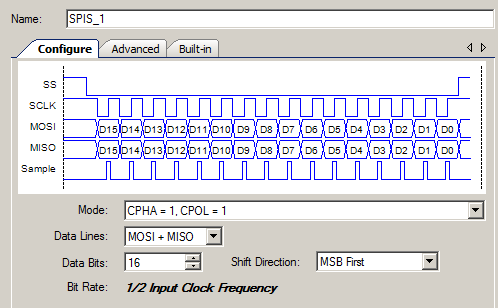
\includegraphics[scale=0.6]{tex/Design/SPI/Clock_mode_SPI}
\caption{Opsætning for SPI forbindelse Devkit8000-PSoC Master}
\end{figure}

Ud fra figur xx, kan det aflæses at SPI clock mode er sat til CPHA = 1 og CPOL = 1, og bitsperword til 16 databits. Det PSoC program som var udleveret blev brugt
som skabelon for gruppens eget program til PSoC master, dog med nogle modifikationer. Især behandlingen af de databits som blev modtaget fra devkittet blev 
genbrugt, da der ikke kunne ændres på disse bits. Koden består dybest set at en interrupt service rutine (ISR), som kaldes hver gang
der modtages data fra devkittet. I ISR er der implementeret en switch, der sørger for at de rigtige metoder kaldes alt efter hvilke databits der modtages.
For mere information omkring koden for PSoC master henvises til bilag(navn på bilag). \\

\textbf{PSoC Master - PSoC Slave:} \\

Til SPI forbindelsen mellem PSoC Master og PSoc slave havde gruppen frie hænder til opsætte SPI. Her blev clock mode valgt til CHPA = 0 og CPOL = 0, og 
bitsperword til 8. Grunden til der kun bliver sendt 8 bits her, er at det er tilstrækkeligt til den simple form for kommunikation der er mellem PSoc enhederne.
8 databits ville også have været fint for Devkit-PSoC forbindelsen, men som tidligere nævnt kunne det ikke ændres da der ikke var adgang til SPI device driveren
på Devkit8000. Clock mode er ændret til default værdien fra PSoC-Creator, og har ikke nogen betydning for kommunikationen så længe begge PSoC enheder har samme
clock mode. Koden for PSoC Slave indeholder ligesom i PSoC master en switch der alt efter de modtagne databits kalder metoder til udførsel af diverse opgaver. 
For mere information omkring koden for PSoC slave henvises til bilag(navn på bilag).   



\subsection{GUI}

Der er mange funktioner i brugergrænsefladen som til at starte med var tiltænkt, som ikke er blevet implementeret. Dette skyldes hovedsageligt 2 ting. Den 
første er at teamet ikke har haft den nødvendige erfaring til at kunne estimere et projekts omfang. Der var rigtig mange ting som blev planlagt som aldrig blev
 udført på grund af mangel på tid. Den anden store grund til at alle funktioner ikke kom med var at gruppen blev nedskåret til en 4 personers gruppe frem for en 
 8 personers grupper som projektet oprindeligt var tiltænkt for. Derfor er det naturligt at gruppen ikke kan nå lige så meget som en gruppe på 8 personer.

De tests som blev udført på brugergrænsefladen var yderst succesfulde, da det ønskede resultat blev opnået. Under testen blev der forsøgt at sende kommandoen 5 
ud igennem SPI, og dette lykkedes som det også fremgår af afsnittet Test.  Det var dog tænkt, og i første omgang implementeret således at brugergrænsefladen kan 
meddele brugeren meddelelse. Dette skulle ske, ved at den fik respons fra PSoC’en, og alt efter hvilken respons den fik, ville den frembringe en dialogboks. Dog 
virkede dette ikke da SPI driveren var ustabil, og ikke ville læse. Istedet blev testen udførst med en virtuel klasse, som kunne simulere modtagelsen af data
fra SPI driveren. Denne test var succesfuld, og derfor kan det konkluderes at GUI implementeringen for statusbeskeder virker som forventet.


\backmatter

%appendix, biblography, index etc here.
\end{document}